% Compact single-column paper/memo format.

\documentclass[10pt,a4paper,parskip=half-]{scrartcl}
\usepackage[margin=1.6cm]{geometry}
\usepackage[T1]{fontenc}
\usepackage[utf8]{inputenc}
\usepackage{lmodern}
\usepackage{amsmath}
\usepackage{amsfonts}
\usepackage{amssymb}
\usepackage{graphicx}
\usepackage{float}
\usepackage{placeins}
\usepackage{booktabs}
\usepackage{array}
\usepackage{adjustbox}
\usepackage{url}
\usepackage{xcolor}
\usepackage{tikz}
\usepackage[nocompress]{cite}
\usepackage{pdflscape}
\usepackage{microtype}
\usepackage{xr}
\externaldocument{main2}
\usetikzlibrary{positioning,arrows.meta,shapes.geometric,fit,backgrounds,calc}
% --- Workflow-overview figure palette (mirrors the Mermaid version in doc/workflow_overview.md) ---
\definecolor{wfIndigo}{HTML}{312E81}
\definecolor{wfIndigoLight}{HTML}{E0E7FF}
\definecolor{wfIndigoMid}{HTML}{4F46E5}
\definecolor{wfAmberDark}{HTML}{D97706}
\definecolor{wfAmberLight}{HTML}{FEF3C7}
\definecolor{wfAmberText}{HTML}{78350F}
\definecolor{wfEmeraldDark}{HTML}{059669}
\definecolor{wfEmeraldLight}{HTML}{D1FAE5}
\definecolor{wfEmeraldText}{HTML}{064E3B}
\definecolor{wfEmeraldBg}{HTML}{ECFDF5}
\definecolor{wfPinkDark}{HTML}{DB2777}
\definecolor{wfPinkLight}{HTML}{FCE7F3}
\definecolor{wfPinkText}{HTML}{831843}
\definecolor{wfBlueDark}{HTML}{2563EB}
\definecolor{wfBlueLight}{HTML}{DBEAFE}
\definecolor{wfBlueText}{HTML}{1E3A8A}
\definecolor{wfBlueBg}{HTML}{EFF6FF}
\definecolor{wfViolet}{HTML}{7C3AED}
\definecolor{wfVioletDark}{HTML}{5B21B6}
\definecolor{wfRoseDark}{HTML}{E11D48}
\definecolor{wfRoseLight}{HTML}{FFE4E6}
\definecolor{wfRoseText}{HTML}{881337}
\definecolor{wfRoseBg}{HTML}{FFF1F2}
\definecolor{wfSlate}{HTML}{475569}
\newcolumntype{L}[1]{>{\raggedright\arraybackslash}p{#1}}
\newcommand{\widecomparisonplot}[1]{\includegraphics[width=0.76\textwidth]{#1}}
\newcommand{\encodingexampleplot}[1]{\includegraphics[width=0.42\linewidth]{#1}}
\newcommand{\subfigtext}[1]{\par\smallskip{\footnotesize #1\par}}
\setlength{\textfloatsep}{8pt plus 2pt minus 2pt}
\setlength{\floatsep}{8pt plus 2pt minus 2pt}
\setlength{\intextsep}{8pt plus 2pt minus 2pt}
\raggedbottom
\hyphenation{op-tical net-works semi-conduc-tor}


\begin{document}
\title{Supplementary Material for\\Controlled Reconstruction of Image-Based Time-Series Encodings}
\author{Adriano~García-Giralda~Milena et al.}
\date{2026}
\maketitle
\renewcommand{\thesection}{S\arabic{section}}
\renewcommand{\thesubsection}{S\arabic{section}.\arabic{subsection}}
\renewcommand{\thetable}{S\arabic{table}}
\renewcommand{\thefigure}{S\arabic{figure}}

\section{Classifier configurations}
\begin{table}[H]
\centering
\caption{Classifier configurations. Each model is trained once per fold on the original (un-reconstructed) windows and reused across all four encodings. Input is $(128,3)$ for the neural models and the flattened $384$-vector for the scikit-learn models; all neural models use the sparse categorical cross-entropy loss.}
\label{tab:classifier_hyperparams}
\small
\begin{tabular}{@{}lp{9.2cm}c@{}}
\toprule
Classifier & Configuration & Seed \\
\midrule
KNN & $k=5$, uniform weights, Minkowski distance ($p=2$) & --- \\
SVM & RBF kernel, $C=1.0$, $\gamma=\text{scale}$ & --- \\
Random Forest & 100 trees, Gini split, unlimited depth, \texttt{max\_features}$=\sqrt{d}$ & 95 \\
LSTM & LSTM(64)\,$\to$\,Dropout(0.2)\,$\to$\,LSTM(32)\,$\to$\,Dropout(0.2)\,$\to$\,Dense-softmax; Adam ($10^{-3}$), 20 epochs, batch 64 & 95 \\
GRU & GRU(64)\,$\to$\,Dropout(0.2)\,$\to$\,GRU(32)\,$\to$\,Dropout(0.2)\,$\to$\,Dense-softmax; Adam ($10^{-3}$), 20 epochs, batch 64 & 95 \\
CNN & Conv1D(196, kernel 16)\,+\,MaxPool(4) concatenated with per-channel statistical features (mean, variance, $\sum|\cdot|$, 10-bin histogram); Dense(1024)\,+\,Dropout(0.05)\,+\,Dense-softmax; $\ell_2=10^{-4}$; Adam ($5\times10^{-4}$), 20 epochs, batch 64 & 95 \\
\bottomrule
\end{tabular}
\end{table}

\section{Encoding sensitivity to signal inversion}
\subsection{Encoding Sensitivity to Signal Inversion}

Before evaluating reconstructions, we first test whether each encoding visually distinguishes a time series from its sign-inverted counterpart. This check is important because an encoding that maps both signals to the same image cannot by itself resolve orientation during reconstruction. The same WISDM window (subject 1600, first walking window, $N=128$) is used for every encoder so the only difference across panels is the encoder itself; the inverted variant negates all three accelerometer channels.

\begin{figure}[H]
    \centering
    \begin{minipage}[b]{0.34\linewidth}
        \centering
        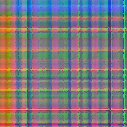
\includegraphics[width=\linewidth]{images/0x0.png}
        \subfigtext{(a) Original}
    \end{minipage}
    \hfill
    \begin{minipage}[b]{0.34\linewidth}
        \centering
        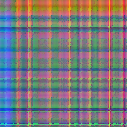
\includegraphics[width=\linewidth]{images/1600x0INV.png}
        \subfigtext{(b) Inverted}
    \end{minipage}
    \caption{Recurrence Plot (RP) images: original vs.\ inverted.}
    \label{fig:INVRP}
\end{figure}

\begin{figure}[H]
    \centering
    \begin{minipage}[b]{0.34\linewidth}
        \centering
        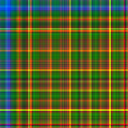
\includegraphics[width=\linewidth]{images/0x0gasf.png}
        \subfigtext{(a) Original}
    \end{minipage}
    \hfill
    \begin{minipage}[b]{0.34\linewidth}
        \centering
        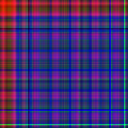
\includegraphics[width=\linewidth]{images/1600x0gasfINV.png}
        \subfigtext{(b) Inverted}
    \end{minipage}
    \caption{Gramian Angular Summation Field (GASF) images: original vs.\ inverted.}
    \label{fig:INVGASF}
\end{figure}

\begin{figure}[H]
    \centering
    \begin{minipage}[b]{0.34\linewidth}
        \centering
        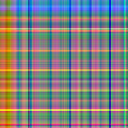
\includegraphics[width=\linewidth]{images/0x0gadf.png}
        \subfigtext{(a) Original}
    \end{minipage}
    \hfill
    \begin{minipage}[b]{0.34\linewidth}
        \centering
        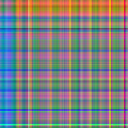
\includegraphics[width=\linewidth]{images/1600x0gadfINV.png}
        \subfigtext{(b) Inverted}
    \end{minipage}
    \caption{Gramian Angular Difference Field (GADF) images: original vs.\ inverted.}
    \label{fig:INVGADF}
\end{figure}

\begin{figure}[H]
    \centering
    \begin{minipage}[b]{0.34\linewidth}
        \centering
        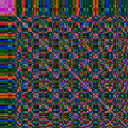
\includegraphics[width=\linewidth]{images/0x0mtf.png}
        \subfigtext{(a) Original}
    \end{minipage}
    \hfill
    \begin{minipage}[b]{0.34\linewidth}
        \centering
        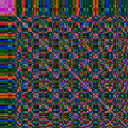
\includegraphics[width=\linewidth]{images/0x0mtfinv.png}
        \subfigtext{(b) Inverted}
    \end{minipage}
    \caption{Markov Transition Field (MTF) images: original vs.\ inverted.}
    \label{fig:INVMTF}
\end{figure}

As illustrated in Figures~\ref{fig:INVRP} (RP) and~\ref{fig:INVGASF} (GASF), the original and inverted time series produce distinctly different images. The same holds for the Gramian Angular Difference Field (Figure~\ref{fig:INVGADF}): negating the input flips the sign of $\sin(\phi_i-\phi_j)$, which after normalisation appears as a contrast inversion of the GADF image. Conversely, as shown in Figure~\ref{fig:INVMTF}, the Markov Transition Field (MTF) yields identical representations for both the original and inverted series, failing to capture their inversion-specific differences. This invariance is \emph{not} because the transition statistics are themselves unchanged: a global sign flip reverses the quantile ranks, $q\mapsto Q{+}1{-}q$, which reverses both the bin ordering and the rows and columns of the transition matrix, $W_{p,q}\mapsto W_{Q+1-p,\,Q+1-q}$. The two reversals cancel at the pixel level --- $M_{a,b}=W_{q_a,q_b}$ maps to $W_{Q+1-(Q+1-q_a),\,Q+1-(Q+1-q_b)}=W_{q_a,q_b}$ --- so the image is left unchanged. The MTF therefore discards the global sign by construction, consistent with the missing sign bit noted in Section~\ref{sec:mtf_reconstruction_method}.

\section{Additional qualitative reconstructions}
\subsection{Qualitative Reconstruction Analysis}
\subsubsection{Artificial Time Series}
For our first experiment, we construct a synthetic time series \( \mathbf{w} \in \mathbb{R}^{N \times 3} \) of length \(N=128\) by sampling an underlying parameter \(t\) uniformly over \([0,\pi]\).  Concretely, define
\[
t_i = \frac{i}{N-1}\,\pi,\qquad i=0,1,\dots,N-1,
\]
and let each vector \(\mathbf{w}_i = [w_{i,0},\,w_{i,1},\,w_{i,2}]^\top\) be given by
\[
w_{i,0} = \cos(t_i),
\qquad
w_{i,1} = \sin(t_i),
\qquad
w_{i,2} = \sin(t_i)\;-\;\cos(t_i).
\]
Thus the full data matrix is
\[
\mathbf{w} =
\begin{bmatrix}
\cos(t_0) & \sin(t_0) & \sin(t_0)-\cos(t_0) \\
\cos(t_1) & \sin(t_1) & \sin(t_1)-\cos(t_1) \\
\vdots    & \vdots    & \vdots             \\
\cos(t_{N-1}) & \sin(t_{N-1}) & \sin(t_{N-1})-\cos(t_{N-1})
\end{bmatrix}.
\]
This three-dimensional signal, composed of a pure cosine channel, a pure sine channel, and their difference, serves as a controlled sanity check for the RP, GASF, GADF, and MTF reconstructions. It is not intended to represent the full WISDM distribution; instead, it provides a visually interpretable case where phase, amplitude, and orientation errors are easy to detect. To keep the evidence separated, every figure in this subsection refers only to the artificial control signal. Figure~\ref{fig:artificial_encodings} shows the image encodings of the three artificial channels under each of the four techniques (RP is $127\times127$ because of the $N-1$ pair embedding; the others are $128\times128$).

\begin{figure}[H]
    \centering
    \begin{minipage}[b]{0.24\linewidth}
        \centering
        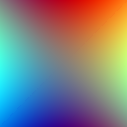
\includegraphics[width=\linewidth]{images/COSRP.png}
        \subfigtext{(a) RP}
    \end{minipage}\hfill
    \begin{minipage}[b]{0.24\linewidth}
        \centering
        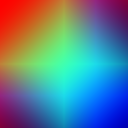
\includegraphics[width=\linewidth]{images/COSGasf.png}
        \subfigtext{(b) GASF}
    \end{minipage}\hfill
    \begin{minipage}[b]{0.24\linewidth}
        \centering
        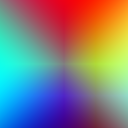
\includegraphics[width=\linewidth]{images/COSgadf.png}
        \subfigtext{(c) GADF}
    \end{minipage}\hfill
    \begin{minipage}[b]{0.24\linewidth}
        \centering
        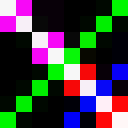
\includegraphics[width=\linewidth]{images/COSmtf.png}
        \subfigtext{(d) MTF}
    \end{minipage}
    \caption{Image encodings of the same artificial three-channel signal (cosine, sine, sine$-$cosine) under each technique.}
    \label{fig:artificial_encodings}
\end{figure}
After generating the encoded images, we decode them and compare the reconstructed series graphically.
\begin{figure}[H]
    \centering
    \widecomparisonplot{images/Comparison_all_wideRP.png}
    \caption{RP reconstruction on the artificial triaxial time series.}
    \label{fig:rp_comparison_artificial}
\end{figure}

\begin{figure}[H]
    \centering
    \widecomparisonplot{images/Comparison_all_wideGAF.png}
    \caption{GASF reconstruction on the artificial triaxial time series.}
    \label{fig:gaf_comparison_artificial}
\end{figure}

\begin{figure}[H]
    \centering
    \widecomparisonplot{images/Comparison_all_wideGADF.png}
    \caption{GADF reconstruction on the artificial triaxial time series.}
    \label{fig:gadf_comparison_artificial}
\end{figure}

\begin{figure}[H]
    \centering
    \widecomparisonplot{images/Comparison_all_widemtf.png}
    \caption{MTF reconstruction on the artificial triaxial time series.}
    \label{fig:mtf_comparison_artificial}
\end{figure}
After encoding the artificial time series (Figure~\ref{fig:artificial_encodings}), we reconstruct each representation and overlay it with the original signal. In this controlled example, the RP comparison (Figure~\ref{fig:rp_comparison_artificial}) overlays the original almost exactly, recovering both shape and amplitude. The GASF comparison (Figure~\ref{fig:gaf_comparison_artificial}) is visually closest to the original in all three channels under the tested normalization. The GADF comparison (Figure~\ref{fig:gadf_comparison_artificial}) is likewise near-perfect: the multi-pivot, boundary-anchored reconstruction overlays the cosine, sine and sin$-$cos channels almost exactly, confirming that the restricted-branch inverse recovers the synthetic signal up to image quantisation. By contrast, the MTF comparison (Figure~\ref{fig:mtf_comparison_artificial}) reveals two limitations that also matter in real data: possible orientation inversion and discretization errors caused by the four transition bins.

\FloatBarrier
\subsubsection{WISDM Sample \texttt{1600$\times$0}}

To assess encoding--decoding fidelity on real sensor data, we selected sample \texttt{1600$\times$0} from fold 0 of the WISDM training set (class~0, Walking, $N=128$ samples). This example is used for qualitative interpretation only; aggregate claims are based on the quantitative tables that follow. Figure~\ref{fig:train0_encodings} shows the encoded images of \emph{the same time-series window} under each of the four encoding techniques, with the three accelerometer axes (\emph{x}, \emph{y}, \emph{z}) mapped to the red/green/blue channels of the image. The RP image is $127\times127$ because the modified definition $s_j=(x_j,x_{j+1})$ embeds the window into $N-1$ adjacent states; GASF, GADF, and MTF are $128\times128$.

\begin{figure}[H]
    \centering
    \begin{minipage}[t]{0.24\linewidth}
        \centering
        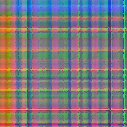
\includegraphics[width=\linewidth]{images/1600xtrp0.png}
        \subfigtext{(a) Recurrence Plot (RP)}
    \end{minipage}\hfill
    \begin{minipage}[t]{0.24\linewidth}
        \centering
        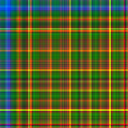
\includegraphics[width=\linewidth]{images/1600x0tgasf.png}
        \subfigtext{(b) GASF}
    \end{minipage}\hfill
    \begin{minipage}[t]{0.24\linewidth}
        \centering
        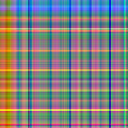
\includegraphics[width=\linewidth]{images/1600x0tgadf.png}
        \subfigtext{(c) GADF}
    \end{minipage}\hfill
    \begin{minipage}[t]{0.24\linewidth}
        \centering
        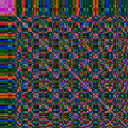
\includegraphics[width=\linewidth]{images/1600x0tmtf.png}
        \subfigtext{(d) Markov Transition Field (MTF)}
    \end{minipage}
    \caption{The four image encodings of the same WISDM window \texttt{1600$\times$0} (fold-0 train, Walking). Per-axis (x,y,z) intensities are stacked as the (R,G,B) channels of each image.}
    \label{fig:train0_encodings}
\end{figure}

After encoding, each image is decoded back into a three-axis time series and overlaid on the original signal. Figures~\ref{fig:rp_comparison_wisdm}--\ref{fig:mtf_comparison_global} present the global comparison across all four encoders (RP, GASF, GADF, MTF).

\begin{figure}[H]
    \centering
    \widecomparisonplot{images/rp_sample_0_global.png}
    \caption{Original vs.\ RP reconstruction for sample \texttt{1600$\times$0}.}
    \label{fig:rp_comparison_wisdm}
\end{figure}

\begin{figure}[H]
    \centering
    \widecomparisonplot{images/gaf_sample_0_global.png}
    \caption{Original vs.\ GASF reconstruction for sample \texttt{1600$\times$0}.}
    \label{fig:gaf_comparison_wisdm}
\end{figure}

\begin{figure}[H]
    \centering
    \widecomparisonplot{images/gadf_sample_0_global.png}
    \caption{Original vs.\ GADF reconstruction for sample \texttt{1600$\times$0}.}
    \label{fig:gadf_comparison_wisdm}
\end{figure}

\begin{figure}[H]
    \centering
    \widecomparisonplot{images/mtf_sample_0_global.png}
    \caption{Original vs.\ MTF reconstruction for sample \texttt{1600$\times$0}.}
    \label{fig:mtf_comparison_global}
\end{figure}

Across the four evaluated methods, RP, GASF, and GADF are visually near-indistinguishable from the original, consistent with their near-original pointwise errors and the utility result discussed in Section~\ref{sec:disc_pointwise}. MTF (Fig.~\ref{fig:mtf_comparison_global}), despite using only four quantised transition levels, captures coarse shape but shows larger deviations where neighbouring transition states are difficult to order.

For clarity, Figures~\ref{fig:mtf_x}--\ref{fig:mtf_z} split the MTF comparison per axis:

\begin{figure}[H]
    \centering
    \widecomparisonplot{images/mtf_sample_0_x_comp.png}
    \caption{Original vs.\ MTF reconstruction for sample \texttt{1600$\times$0}, axis \emph{x}.}
    \label{fig:mtf_x}
\end{figure}

\begin{figure}[H]
    \centering
    \widecomparisonplot{images/mtf_sample_0_y_comp.png}
    \caption{Original vs.\ MTF reconstruction for sample \texttt{1600$\times$0}, axis \emph{y}.}
    \label{fig:mtf_y}
\end{figure}

\begin{figure}[H]
    \centering
    \widecomparisonplot{images/mtf_sample_0_z_comp.png}
    \caption{Original vs.\ MTF reconstruction for sample \texttt{1600$\times$0}, axis \emph{z}.}
    \label{fig:mtf_z}
\end{figure}

\FloatBarrier

\section{Additional spectral-fidelity metrics}

The main article separates spectral shape from total energy. Table~\ref{tab:supp_spectral_energy} reports the complementary quantities omitted from the compact body table. Energy error is the relative difference in total Welch power; band-shape error is the mean absolute difference in normalised spectral mass over 0--1, 1--3, 3--5, and 5--10\,Hz. Neither quantity is folded into the PSD-shape distance.

\begin{table}[H]
\centering
\caption{Complementary spectral metrics over 8,172 windows (mean$\pm$std across windows, averaged over axes).}
\label{tab:supp_spectral_energy}
\begin{tabular}{lcc}
\toprule
Method & Relative total-energy error & Band-shape error \\
\midrule
RP   & $0.0029\pm0.0026$ & $0.00020\pm0.00022$ \\
GASF & $0.0054\pm0.0055$ & $0.00085\pm0.00085$ \\
GADF & $0.0011\pm0.0009$ & $0.00029\pm0.00021$ \\
MTF  & $2.199\pm8.844$   & $0.05624\pm0.03692$ \\
\bottomrule
\end{tabular}
\end{table}

\section{Robustness details and error attribution}
\label{sec:supp_robustness}

The local-stability sample is selected deterministically from window-level fold~0 (seed 0): 30 windows from each of the five activities, using round-robin sampling over the available subjects within each activity. The resulting 150 windows cover all 51 subjects. Fold~0 is only a reproducible sampling frame here: the decoders are untrained and no configuration is selected on this sample. For every nonzero noise level, two independent arrays are sampled over all pixels and channels, clipped to $[0,255]$, rounded to the 8-bit grid, and decoded; replicate errors are averaged within each window. Two draws per level are enough to average out the leading per-window replicate variation but do not fully characterise the noise distribution at a window; accordingly, the reported standard deviations and intervals summarise variability \emph{across} windows, and the number of draws is exposed as \texttt{TFG\_ROBUST\_REPS} so the curve can be recomputed with more realizations. The subject-cluster intervals in Table~\ref{tab:supp_robustness_ci} resample the 51 represented subjects as whole clusters. The MTF encoder emitted tied-quantile warnings for some axis-series; allowing fewer distinct bins in those cases is part of the evaluated quantisation behaviour.

\begin{table}[H]
\centering
\caption{Subject-cluster bootstrap 95\% intervals for mean NMAE along the perturbation curves ($10^4$ resamples). These accompany the between-window standard deviations in the main article.}
\label{tab:supp_robustness_ci}
\small
\resizebox{\textwidth}{!}{%
\begin{tabular}{lccccc}
\toprule
Method & $\sigma=0$ & $\sigma=2$ & $\sigma=4$ & $\sigma=8$ & $\sigma=16$ \\
\midrule
RP   & $[0.0010,0.0012]$ & $[0.0040,0.0050]$ & $[0.0076,0.0092]$ & $[0.0155,0.0187]$ & $[0.0317,0.0364]$ \\
GASF & $[0.0014,0.0015]$ & $[0.0124,0.0137]$ & $[0.0207,0.0222]$ & $[0.0349,0.0368]$ & $[0.0621,0.0647]$ \\
GADF & $[0.0011,0.0013]$ & $[0.0071,0.0077]$ & $[0.0142,0.0153]$ & $[0.0304,0.0327]$ & $[0.0644,0.0696]$ \\
MTF  & $[0.2686,0.2950]$ & $[0.2733,0.2963]$ & $[0.2752,0.2991]$ & $[0.2726,0.2956]$ & $[0.2694,0.2903]$ \\
\bottomrule
\end{tabular}
}
\end{table}

The cycle residual is the relative Frobenius error defined in the main article and compares native float operator matrices, not PNG intensities. Table~\ref{tab:supp_cycle_gate} also reports the maximum wiring-gate discrepancy over the sample. All four clean reconstructions agree numerically with their cached pipeline counterparts on every window; ``passed'' means the per-window maximum is below the stated 0.05 threshold, not that the threshold itself is an exactness claim.

\begin{table}[H]
\centering
\caption{Self-consistency gate and clean image-domain cycle residual (mean$\pm$standard deviation and subject-cluster bootstrap 95\% interval).}
\label{tab:supp_cycle_gate}
\begin{tabular}{lccc}
\toprule
Method & Maximum gate NMAE & Cycle residual & Cycle 95\% interval \\
\midrule
RP   & $<10^{-8}$ & $0.0502\pm0.0294$ & $[0.0465,0.0539]$ \\
GASF & $<10^{-8}$ & $0.0046\pm0.0012$ & $[0.0045,0.0048]$ \\
GADF & $<10^{-8}$ & $0.0044\pm0.0016$ & $[0.0042,0.0046]$ \\
MTF  & $<10^{-8}$ & $0.1242\pm0.1955$ & $[0.0946,0.1556]$ \\
\bottomrule
\end{tabular}
\end{table}

Table~\ref{tab:error_sources} uses each method's native float operator matrix before any 8-bit storage map. This resolves the earlier GADF discrepancy: its restricted-branch inverse is exact to numerical precision in this path. RP is different; its small float error is algorithmic, so PNG quantisation is the dominant, but not the only, source of its clean-round-trip error.

\begin{table}[H]
\centering
\caption{Reconstruction NMAE by source over the same 150 windows (mean$\pm$standard deviation): native float operator, clean 8-bit PNG round trip, and perturbed PNG at $\sigma=8$.}
\label{tab:error_sources}
\begin{tabular}{lccc}
\toprule
Method & Native float operator & 8-bit PNG & Perturbed ($\sigma=8$) \\
\midrule
RP   & $0.00036\pm0.00029$ & $0.0011\pm0.0007$ & $0.0170\pm0.0090$ \\
GASF & $<10^{-12}$          & $0.0015\pm0.0003$ & $0.0358\pm0.0061$ \\
GADF & $<10^{-12}$          & $0.0012\pm0.0004$ & $0.0315\pm0.0079$ \\
MTF  & $0.2819\pm0.0830$   & $0.2812\pm0.0836$ & $0.2838\pm0.0787$ \\
\bottomrule
\end{tabular}
\end{table}

\section{Complete reconstruction results by fold}
\begin{table}[H]
\centering
\caption{Per-fold reconstruction error for both 3-fold protocols (physical units, m/s$^2$). Each cell is the per-window global metric (averaged over the three axes) averaged over that fold's test windows. Because the decoders are deterministic and untrained, a window reconstructs identically in any fold; the two protocols only repartition the same $8172$ windows, so the Pooled column is identical for both and equals the full-dataset value of Table~\ref{tab:pointwise_pooled}. The window-level folds are near-identical stratified partitions (negligible fold-to-fold spread), whereas the subject-out folds vary more because different subjects are held out.}
\label{tab:pointwise_perfold}
\resizebox{\textwidth}{!}{%
\begin{tabular}{ll ccc ccc c}
\toprule
 & & \multicolumn{3}{c}{\textbf{Window-level 3-fold}} & \multicolumn{3}{c}{\textbf{Subject-out 3-fold}} & \\
\cmidrule(lr){3-5}\cmidrule(lr){6-8}
\textbf{Encoder} & \textbf{Metric} & F0 & F1 & F2 & F0 & F1 & F2 & \textbf{Pooled} \\
\midrule
\textbf{RP} & MAE & $0.0148$ & $0.0149$ & $0.0149$ & $0.0142$ & $0.0155$ & $0.0147$ & $0.0148$ \\
 & MSE & $0.0009$ & $0.0011$ & $0.0011$ & $0.0009$ & $0.0011$ & $0.0010$ & $0.0010$ \\
 & Pearson & $0.99998$ & $0.99998$ & $0.99998$ & $0.99998$ & $0.99998$ & $0.99998$ & $0.99998$ \\
\midrule
\textbf{GASF} & MAE & $0.0202$ & $0.0205$ & $0.0207$ & $0.0189$ & $0.0211$ & $0.0214$ & $0.0205$ \\
 & MSE & $0.0042$ & $0.0043$ & $0.0044$ & $0.0037$ & $0.0041$ & $0.0051$ & $0.0043$ \\
 & Pearson & $0.99988$ & $0.99988$ & $0.99988$ & $0.99988$ & $0.99988$ & $0.99988$ & $0.99988$ \\
\midrule
\textbf{GADF} & MAE & $0.0156$ & $0.0157$ & $0.0159$ & $0.0147$ & $0.0162$ & $0.0163$ & $0.0157$ \\
 & MSE & $0.0008$ & $0.0008$ & $0.0008$ & $0.0007$ & $0.0008$ & $0.0009$ & $0.0008$ \\
 & Pearson & $0.99999$ & $0.99999$ & $0.99999$ & $0.99999$ & $0.99999$ & $0.99999$ & $0.99999$ \\
\midrule
\textbf{MTF} & MAE & $3.98$ & $3.94$ & $3.91$ & $3.71$ & $4.04$ & $4.07$ & $3.94$ \\
 & MSE & $56.42$ & $55.25$ & $54.62$ & $48.13$ & $52.54$ & $65.43$ & $55.43$ \\
 & Pearson & $0.00289$ & $0.02089$ & $0.01689$ & $0.00977$ & $0.00116$ & $0.02982$ & $0.01356$ \\
\bottomrule
\end{tabular}
}
\end{table}

\section{Complete grouped subject-out classifier results}
\begin{table}[H]
\centering
\caption{Grouped subject-out three-fold accuracies for all six classifiers (mean$\pm$standard deviation across folds). The folds contain disjoint groups of 16, 18, and 17 test subjects.}
\label{tab:gadf_summary_perfold_subject_out}
\setlength{\tabcolsep}{5pt}
\footnotesize
\begin{tabular}{lccccc}
\toprule
Classifier & Original & RP & GASF & GADF & MTF \\
\midrule
KNN  & $0.504\pm0.035$ & $0.504\pm0.035$ & $0.504\pm0.034$ & $0.505\pm0.034$ & $0.465\pm0.039$ \\
SVM  & $0.738\pm0.020$ & $0.739\pm0.020$ & $0.738\pm0.020$ & $0.738\pm0.020$ & $0.665\pm0.026$ \\
RF   & $0.786\pm0.039$ & $0.786\pm0.039$ & $0.787\pm0.039$ & $0.787\pm0.039$ & $0.689\pm0.026$ \\
LSTM & $0.744\pm0.029$ & $0.744\pm0.028$ & $0.744\pm0.029$ & $0.744\pm0.028$ & $0.672\pm0.035$ \\
GRU  & $0.811\pm0.026$ & $0.811\pm0.026$ & $0.811\pm0.026$ & $0.811\pm0.026$ & $0.702\pm0.025$ \\
CNN  & $0.794\pm0.050$ & $0.794\pm0.049$ & $0.794\pm0.050$ & $0.794\pm0.050$ & $0.684\pm0.031$ \\
\bottomrule
\end{tabular}
\end{table}

\section{Window-level vs subject-out accuracy}
\label{sec:supp_window_vs_subject}
Table~\ref{tab:window_vs_subject_out} places the window-level (W, within-distribution) and grouped subject-out (S, primary) accuracies side by side for the three representative classifiers reported in the main text. Absolute accuracy is higher under the window-level split, as expected when windows of a test subject may also appear in training, but the encoder ranking is identical under both protocols: RP, GASF and GADF track the original signal, while MTF degrades every classifier. The main text reports the subject-out column only.

\begin{table}[H]
\centering
\caption{Window-level (W) vs grouped subject-out (S) three-fold accuracy (mean across folds) for three representative classifiers. The encoder ranking is identical under both protocols.}
\label{tab:window_vs_subject_out}
\resizebox{\textwidth}{!}{%
\begin{tabular}{l|cc|cc|cc|cc|cc}
\toprule
 & \multicolumn{2}{c|}{Original} & \multicolumn{2}{c|}{RP} & \multicolumn{2}{c|}{GASF} & \multicolumn{2}{c|}{GADF} & \multicolumn{2}{c}{MTF} \\
Classifier & W & S & W & S & W & S & W & S & W & S \\
\midrule
CNN  & 0.901 & 0.794 & 0.901 & 0.794 & 0.901 & 0.794 & 0.901 & 0.794 & 0.758 & 0.684 \\
GRU  & 0.923 & 0.811 & 0.923 & 0.811 & 0.923 & 0.811 & 0.923 & 0.811 & 0.765 & 0.702 \\
RF   & 0.891 & 0.786 & 0.892 & 0.786 & 0.891 & 0.787 & 0.892 & 0.787 & 0.757 & 0.689 \\
\bottomrule
\end{tabular}}
\end{table}

\section{Subject-level classification equivalence}
\label{sec:supp_equivalence}

\paragraph*{Simultaneous max-deviation bootstrap algorithm.}
The central equivalence result is a joint subject-cluster bootstrap. Because it is the headline statistic, we state the exact procedure. Let a \emph{family} be a set of $C$ comparisons (here $C=18$ for the primary RP/GASF/GADF family, $C=6$ for the separate MTF control family), each a fixed (classifier, encoder) pair, evaluated over the same $K=51$ subjects in a fixed order.
\begin{enumerate}
\item \textbf{Per-subject differences.} For subject $s$ and comparison $c$, compute the per-subject accuracy difference $\Delta_{c,s}=\mathrm{acc}^{\mathrm{orig}}_{s}-\mathrm{acc}^{\mathrm{recon}(c)}_{s}$, where each subject accuracy is that subject's fraction of correctly classified held-out windows (under subject-out validation every subject is a test subject in exactly one outer fold). This gives a $K\times C$ matrix with one row per subject.
\item \textbf{Point estimates.} The estimate for comparison $c$ is the subject mean $\hat\mu_c=\frac1K\sum_s\Delta_{c,s}$ (the ``mean $\Delta$acc'' column). Subjects, not windows, are the sampling unit; no per-subject weighting or standardisation is applied.
\item \textbf{Joint resampling.} For $b=1,\dots,B$ ($B=10^4$) draw one index vector of $K$ subjects with replacement and apply the \emph{same} vector to every column, so whole subjects are resampled jointly and the dependence between classifiers and encodings is preserved. Compute the resampled means $\hat\mu^{(b)}_c$ for all $c$.
\item \textbf{Family-wise critical value.} Centre each resampled mean on its point estimate, $d^{(b)}_c=\hat\mu^{(b)}_c-\hat\mu_c$ (raw accuracy units; the deviations are \emph{not} studentised or divided by a bootstrap standard error), take the family maximum $D^{(b)}=\max_c|d^{(b)}_c|$, and set the single critical value $\kappa$ to the $95$th percentile of $\{D^{(b)}\}_{b=1}^{B}$. One $\kappa$ is shared by all comparisons in the family, which is what makes the coverage simultaneous rather than pointwise.
\item \textbf{Intervals and decision.} The simultaneous interval for comparison $c$ is $[\hat\mu_c-\kappa,\;\hat\mu_c+\kappa]$. Equivalence at margin $m$ is declared iff that whole interval lies inside $[-m,+m]$; the main text uses $m=0.01$ with $m=0.02$ as a less stringent sensitivity check.
\end{enumerate}
Each family uses an independent random seed and its own $\kappa$; no resamples or critical values are shared between the primary and MTF families, and none are pooled across the subject-out and window-level protocols. The ``interval span'' reported in the compact main-text table is the union of the $C$ per-comparison intervals within a method and is descriptive only. This is the \texttt{\_cluster\_bootstrap\_simultaneous} routine in \texttt{scripts/\_stat\_tests.py}; the confirmatory paired TOST uses the same per-subject $\Delta_{c,s}$ but a Student-$t$ interval at the bilateral $90\%$ level, so the simultaneous $95\%$ bootstrap is the stricter of the two.

Table~\ref{tab:supp_equivalence_individual} exposes every classifier-specific simultaneous interval hidden by the compact span in the main article. The primary family contains the 18 RP/GASF/GADF comparisons; MTF's six negative-control comparisons form a separate family. Within each family, all classifiers share the same $10^4$ subject resamples and the same bootstrap maximum-deviation critical value. Thus these are simultaneous intervals, not six unadjusted pointwise intervals and not an ``envelope CI.''

\begin{table}[H]
\centering
\caption{Mean per-subject $\Delta$accuracy and simultaneous 95\% interval, Original $-$ reconstruction, under grouped subject-out validation (51 subjects). Bold cells lie wholly inside $[-0.01,+0.01]$.}
\label{tab:supp_equivalence_individual}
\footnotesize
\setlength{\tabcolsep}{3pt}
\resizebox{\textwidth}{!}{%
\begin{tabular}{lcccc}
\toprule
Classifier & RP & GASF & GADF & MTF \\
\midrule
KNN & $\mathbf{+0.0003\ [-0.0019,+0.0024]}$ & $\mathbf{-0.0001\ [-0.0022,+0.0021]}$ & $\mathbf{-0.0005\ [-0.0027,+0.0016]}$ & $+0.0474\ [+0.0209,+0.0739]$ \\
SVM & $\mathbf{-0.0001\ [-0.0022,+0.0020]}$ & $\mathbf{+0.0000\ [-0.0021,+0.0021]}$ & $\mathbf{+0.0008\ [-0.0013,+0.0030]}$ & $+0.0651\ [+0.0385,+0.0916]$ \\
RF  & $\mathbf{+0.0012\ [-0.0009,+0.0033]}$ & $\mathbf{-0.0006\ [-0.0027,+0.0016]}$ & $\mathbf{-0.0002\ [-0.0023,+0.0019]}$ & $+0.0910\ [+0.0645,+0.1176]$ \\
LSTM & $\mathbf{+0.0004\ [-0.0017,+0.0025]}$ & $\mathbf{-0.0000\ [-0.0022,+0.0021]}$ & $\mathbf{+0.0001\ [-0.0020,+0.0022]}$ & $+0.0697\ [+0.0432,+0.0963]$ \\
GRU & $\mathbf{-0.0002\ [-0.0023,+0.0019]}$ & $\mathbf{-0.0002\ [-0.0023,+0.0020]}$ & $\mathbf{-0.0003\ [-0.0024,+0.0019]}$ & $+0.1124\ [+0.0858,+0.1389]$ \\
CNN & $\mathbf{+0.0004\ [-0.0017,+0.0025]}$ & $\mathbf{-0.0002\ [-0.0024,+0.0019]}$ & $\mathbf{-0.0001\ [-0.0023,+0.0020]}$ & $+0.1102\ [+0.0837,+0.1368]$ \\
\bottomrule
\end{tabular}
}
\end{table}

For completeness, Table~\ref{tab:supp_equivalence_protocols} applies the same simultaneous procedure to a separate 18-comparison family under the secondary window-level protocol (and a separate six-comparison MTF family). No interval is pooled across protocols. Both protocols yield the same equivalence decisions.

\begin{table}[H]
\centering
\caption{Descriptive spans of classifier-specific simultaneous 95\% intervals by protocol. Each protocol is analysed as a separate family; the displayed span is not itself a confidence interval.}
\label{tab:supp_equivalence_protocols}
\small
\setlength{\tabcolsep}{4pt}
\begin{tabular}{lccc ccc}
\toprule
 & \multicolumn{3}{c}{Window-level (secondary)} & \multicolumn{3}{c}{Subject-out (primary)} \\
\cmidrule(lr){2-4}\cmidrule(lr){5-7}
Method & Mean $\Delta$ range & Interval span & Eq.\,$\pm0.01$ & Mean $\Delta$ range & Interval span & Eq.\,$\pm0.01$ \\
\midrule
RP   & $[-0.0009,+0.0004]$ & $[-0.0032,+0.0027]$ & 6/6 & $[-0.0002,+0.0012]$ & $[-0.0023,+0.0033]$ & 6/6 \\
GASF & $[-0.0003,+0.0005]$ & $[-0.0026,+0.0028]$ & 6/6 & $[-0.0006,+0.0000]$ & $[-0.0027,+0.0021]$ & 6/6 \\
GADF & $[-0.0006,+0.0002]$ & $[-0.0029,+0.0025]$ & 6/6 & $[-0.0005,+0.0008]$ & $[-0.0027,+0.0030]$ & 6/6 \\
MTF  & $[+0.0819,+0.1542]$ & $[+0.0550,+0.1812]$ & 0/6 & $[+0.0474,+0.1124]$ & $[+0.0209,+0.1389]$ & 0/6 \\
\bottomrule
\end{tabular}
\end{table}

\section{Extended RP ablation}

Table~\ref{tab:supp_rp_ablation} separates the RP operator-range round trip from the geometric choices. Correct inverse normalisation restores a predominantly two-dimensional Euclidean spectrum; both the full state geometry and signed orientation are necessary for near-lossless reconstruction.

\begin{table}[H]
\centering
\caption{RP ablation on 100 stratified fold-0 windows. $\mathrm{EVR}_2$ is the MDS variance in the two leading positive dimensions.}
\label{tab:supp_rp_ablation}
\begin{tabular}{lccc}
\toprule
Variant & MAE & Pearson & $\mathrm{EVR}_2$ \\
\midrule
2-D MDS + signed orientation & \textbf{0.010} & \textbf{1.000} & 0.947 \\
Signal-range decode (incorrect) & 1.047 & 0.959 & 0.218 \\
Without signed orientation & 2.033 & 0.794 & 0.947 \\
Prior one-dimensional graph decoder & 2.177 & 0.918 & 0.730 \\
\bottomrule
\end{tabular}
\end{table}

\section{Extended GADF pivot sweep}
\paragraph*{Pivot-ensemble size.}
Averaging the reconstruction over the $n_p$ most-central rows, rather than trusting a single pivot, is the second numeric choice. Table~\ref{tab:supp_gadf_npivots} sweeps $n_p$ on the same PNG round trip at $\alpha=0.7$: the pointwise error falls monotonically --- more than halving from a single pivot ($0.0353$) to five ($0.0158$, the value used throughout the paper) and improving further to $0.0119$ at $n_p=9$ --- at essentially constant cost ($1.54$--$1.59$\,ms per axis-series), since each extra pivot is one more $O(N)$ pass over an already-loaded matrix. We fix $n_p=5$ as a conservative default that captures most of the averaging gain; a larger ensemble would lower the reported GADF error further at negligible extra cost, but $n_p$ is kept fixed so the headline numbers are not tuned on the evaluation windows.

\begin{table}[!htbp]
\centering
\caption{GADF pivot-ensemble sweep on the same $1\,500$ WISDM windows ($4\,500$ axis-series) at $\alpha=0.7$. $n_p$ is the number of averaged central pivot rows; MAE is the 8-bit PNG round-trip error in physical units; time is per axis-series. The default used everywhere else in the paper is $n_p=5$.}
\label{tab:supp_gadf_npivots}
\setlength{\tabcolsep}{8pt}
\footnotesize
\begin{tabular}{cccccc}
\toprule
$n_p$ & 1 & 3 & 5 & 7 & 9 \\
\midrule
MAE (8-bit PNG) & $0.0353$ & $0.0206$ & $\mathbf{0.0158}$ & $0.0134$ & $0.0119$ \\
Time (ms/axis)  & $1.54$ & $1.55$ & $1.57$ & $1.58$ & $1.59$ \\
\bottomrule
\end{tabular}
\end{table}

\section{Extended MTF ablations}
\paragraph*{Decoder ablation (at fixed $Q=4$).}
We compare four decoder configurations on the same encoded MTF images (Table~\ref{tab:supp_mtf_ablation}): the cosine-pivot ordering heuristic, Fiedler-vector ordering, Fiedler-vector ordering with stored bin-midpoint metadata, and Fiedler-vector ordering with both midpoint metadata and a sign-bit. The encoder is held constant. Bin midpoints (storing $Q$ floats per axis, the median of each quantile bin) and a sign-bit (one bit per axis to disambiguate the mirror symmetry) are \emph{not} part of the side-information contract used for the headline numbers; they characterize the achievable floor that any MTF decoder operating on top of the standard MTF image cannot beat.

\begin{table}[H]
\centering
\caption{MTF decoder ablation at $Q=4$, 100 stratified window-level fold-0 test windows ($T=128$); pointwise MAE and Pearson averaged across the three accelerometer axes.}
\label{tab:supp_mtf_ablation}
\setlength{\tabcolsep}{4pt}
\footnotesize
\begin{tabular}{lcc}
\toprule
Decoder variant & MAE & Pearson \\
\midrule
Cosine-pivot heuristic               & 6.493 & $+0.023$ \\
Fiedler ordering                      & 5.060 & $-0.008$ \\
Fiedler + midpoint metadata           & 3.926 & $+0.013$ \\
Fiedler + midpoint + sign-bit         & 2.603 & $+0.465$ \\
\bottomrule
\end{tabular}
\end{table}

The Fiedler ordering alone, with no extra metadata, drops the cosine-pivot pointwise MAE by 22\% ($6.49\to 5.06$). Adding $Q$ bin-median floats per axis (comparable in cost to the optional per-axis $(\min,\max)$ calibration used only for physical-scale recovery) drops it to $3.93$; adding a single sign-bit per axis -- which resolves the global reversal ambiguity of the inferred Fiedler ordering, though not the many-to-one quantisation and transition-profile ambiguities intrinsic to MTF -- drops it further to $2.60$. We use \emph{Fiedler ordering without midpoint or sign-bit metadata} for every MTF number elsewhere in the paper because it keeps the side-information contract identical to the cosine-pivot heuristic, and characterizes what an MTF decoder can achieve without extra metadata beyond the standard optional per-axis physical-scale calibration.

\paragraph*{Bin-count ablation across $Q$.}
The bin count $Q$ is the parameter most often discussed in the MTF literature. We performed an exploratory sweep of $Q\in\{2,4,6,8,10,16\}$ on the full stratified window-level 3-fold test set ($N=8\,172$ pooled windows; approximately 2\,724 per fold) and evaluated the six-classifier panel on each reconstruction, using the Fiedler decoder uniformly. Because this sweep uses test windows, it is a post-hoc sensitivity analysis, not internal validation and not an unbiased basis for selecting an optimal MTF decoder. Table~\ref{tab:mtf_ablation_q} is retained to disclose that choice.

\begin{table}[!htbp]
\centering
\caption{Exploratory MTF bin-count sensitivity on pooled test windows ($N=8\,172$). Pointwise MAE and Pearson are averaged across axes; classifier accuracies are 3-fold means. Highlighting is descriptive and does not constitute nested model selection.}
\label{tab:mtf_ablation_q}
\setlength{\tabcolsep}{5pt}
\footnotesize
\begin{tabular}{rcc|cccccc}
\toprule
$Q$ & \textbf{MAE} & \textbf{Pearson} & KNN & SVM & RF & LSTM & GRU & CNN \\
\midrule
 2  & 4.11 & $+0.002$ & 0.490 & \textbf{0.705} & \textbf{0.762} & 0.756 & \textbf{0.771} & \textbf{0.774} \\
\textbf{4}  & \textbf{3.95} & $\mathbf{+0.013}$ & \textbf{0.559} & 0.697 & 0.757 & \textbf{0.757} & 0.765 & 0.773 \\
 6  & 4.01 & $+0.004$ & 0.556 & 0.697 & 0.757 & 0.755 & 0.761 & 0.770 \\
 8  & 4.03 & $-0.001$ & 0.539 & 0.695 & 0.753 & 0.757 & 0.764 & 0.765 \\
 10 & 4.07 & $+0.000$ & 0.527 & 0.693 & 0.754 & 0.756 & 0.762 & 0.758 \\
 16 & 4.13 & $-0.014$ & 0.520 & 0.697 & 0.755 & 0.757 & 0.762 & 0.753 \\
\bottomrule
\end{tabular}
\end{table}

Three observations matter:
\begin{enumerate}
\item \textbf{Pointwise fidelity is jointly maximised at $Q=4$.} Both MAE and Pearson reach their optimum at $Q=4$ ($3.95$, $+0.013$); every other choice of $Q$ strictly degrades both metrics. The amplitude of the variation is modest (MAE moves in $[3.95, 4.13]$ across the swept range) because the Fiedler decoder is dominated by the intra-bin variance regardless of $Q$, but the location of the minimum is unambiguous.
\item \textbf{The amplitude-sensitive KNN classifier peaks at $Q=4$.} KNN -- the only classifier in our panel that measures local geometric similarity in the flattened sample space -- improves by $+6.9$ percentage points going from $Q=2$ to $Q=4$ ($0.490\to 0.559$) and then monotonically degrades down to $0.520$ at $Q=16$. CNN, which extracts local temporal patterns through learned convolutional filters, is similar at $Q=2$ and $Q=4$ ($0.774$ vs $0.773$) and decreases moderately for larger $Q$ (to $0.753$ at $Q=16$). KNN, the classifier that most exploits fine-grained amplitude structure, is thus the one that clearly pays for under- or over-quantisation.
\item \textbf{Coarse-pattern classifiers are nearly insensitive to $Q$.} SVM, Random Forest, LSTM and GRU vary by at most $0.012$ accuracy across the entire $Q\in\{2,\ldots,16\}$ sweep, with their (statistically negligible) optimum located at $Q=2$. These four classifiers absorb most of the discriminative signal through bin-transition counts rather than through quantised amplitude shape, which is why they tolerate the coarsest quantisation. Their indifference to $Q$ also explains why MTF as a representation is robust to the choice of $Q$: in the regime where most of the activity signal lives in the transition structure (high-ceiling neural classifiers), MTF's pre-quantisation step is not the bottleneck.
\end{enumerate}

Taken together, the exploratory results explain why $Q=4$ was used in the reported lossy control: it minimises pointwise MAE and maximises pointwise Pearson and KNN accuracy on this pooled sample. They do not establish out-of-subject optimality. A confirmatory comparison would select $Q$ inside a subject-grouped inner loop for every outer fold.

\section{RP--GADF structural diagnostic}
\subsection{Null-Corrected RP/GADF Regional Overlap}
\label{sec:disc_rp_gadf_overlap}

The visual proximity between RP and GADF is easy to overstate from a single example, so we add a diagnostic test that deliberately separates spatial region alignment from marginal colour statistics. On the full set of non-overlapping smartwatch-accelerometer WISDM windows (window length \(N=128\)), we encode the same signal as signed RP and GADF, align the matrices on the common \(127\times127\) support, and quantise each image channel into \(B\) visual intensity ranges. For every matched pair \((\mathrm{RP}_i,\mathrm{GADF}_i)\), we compare the quantised regions against a conservative null pair \((\mathrm{RP}_i,\mathrm{GADF}_j)\), where \(j\neq i\) is drawn from the same activity class. The primary statistic is a weighted regional Jaccard score, \(\sum_b |R_b\cap G_b|/\sum_b |R_b\cup G_b|\), averaged across the grayscale view and the three RGB/axis channels. We also compute a distribution-only overlap that ignores pixel position and a boundary-F1 score between quantised region edges.

\begin{figure}[H]
    \centering
    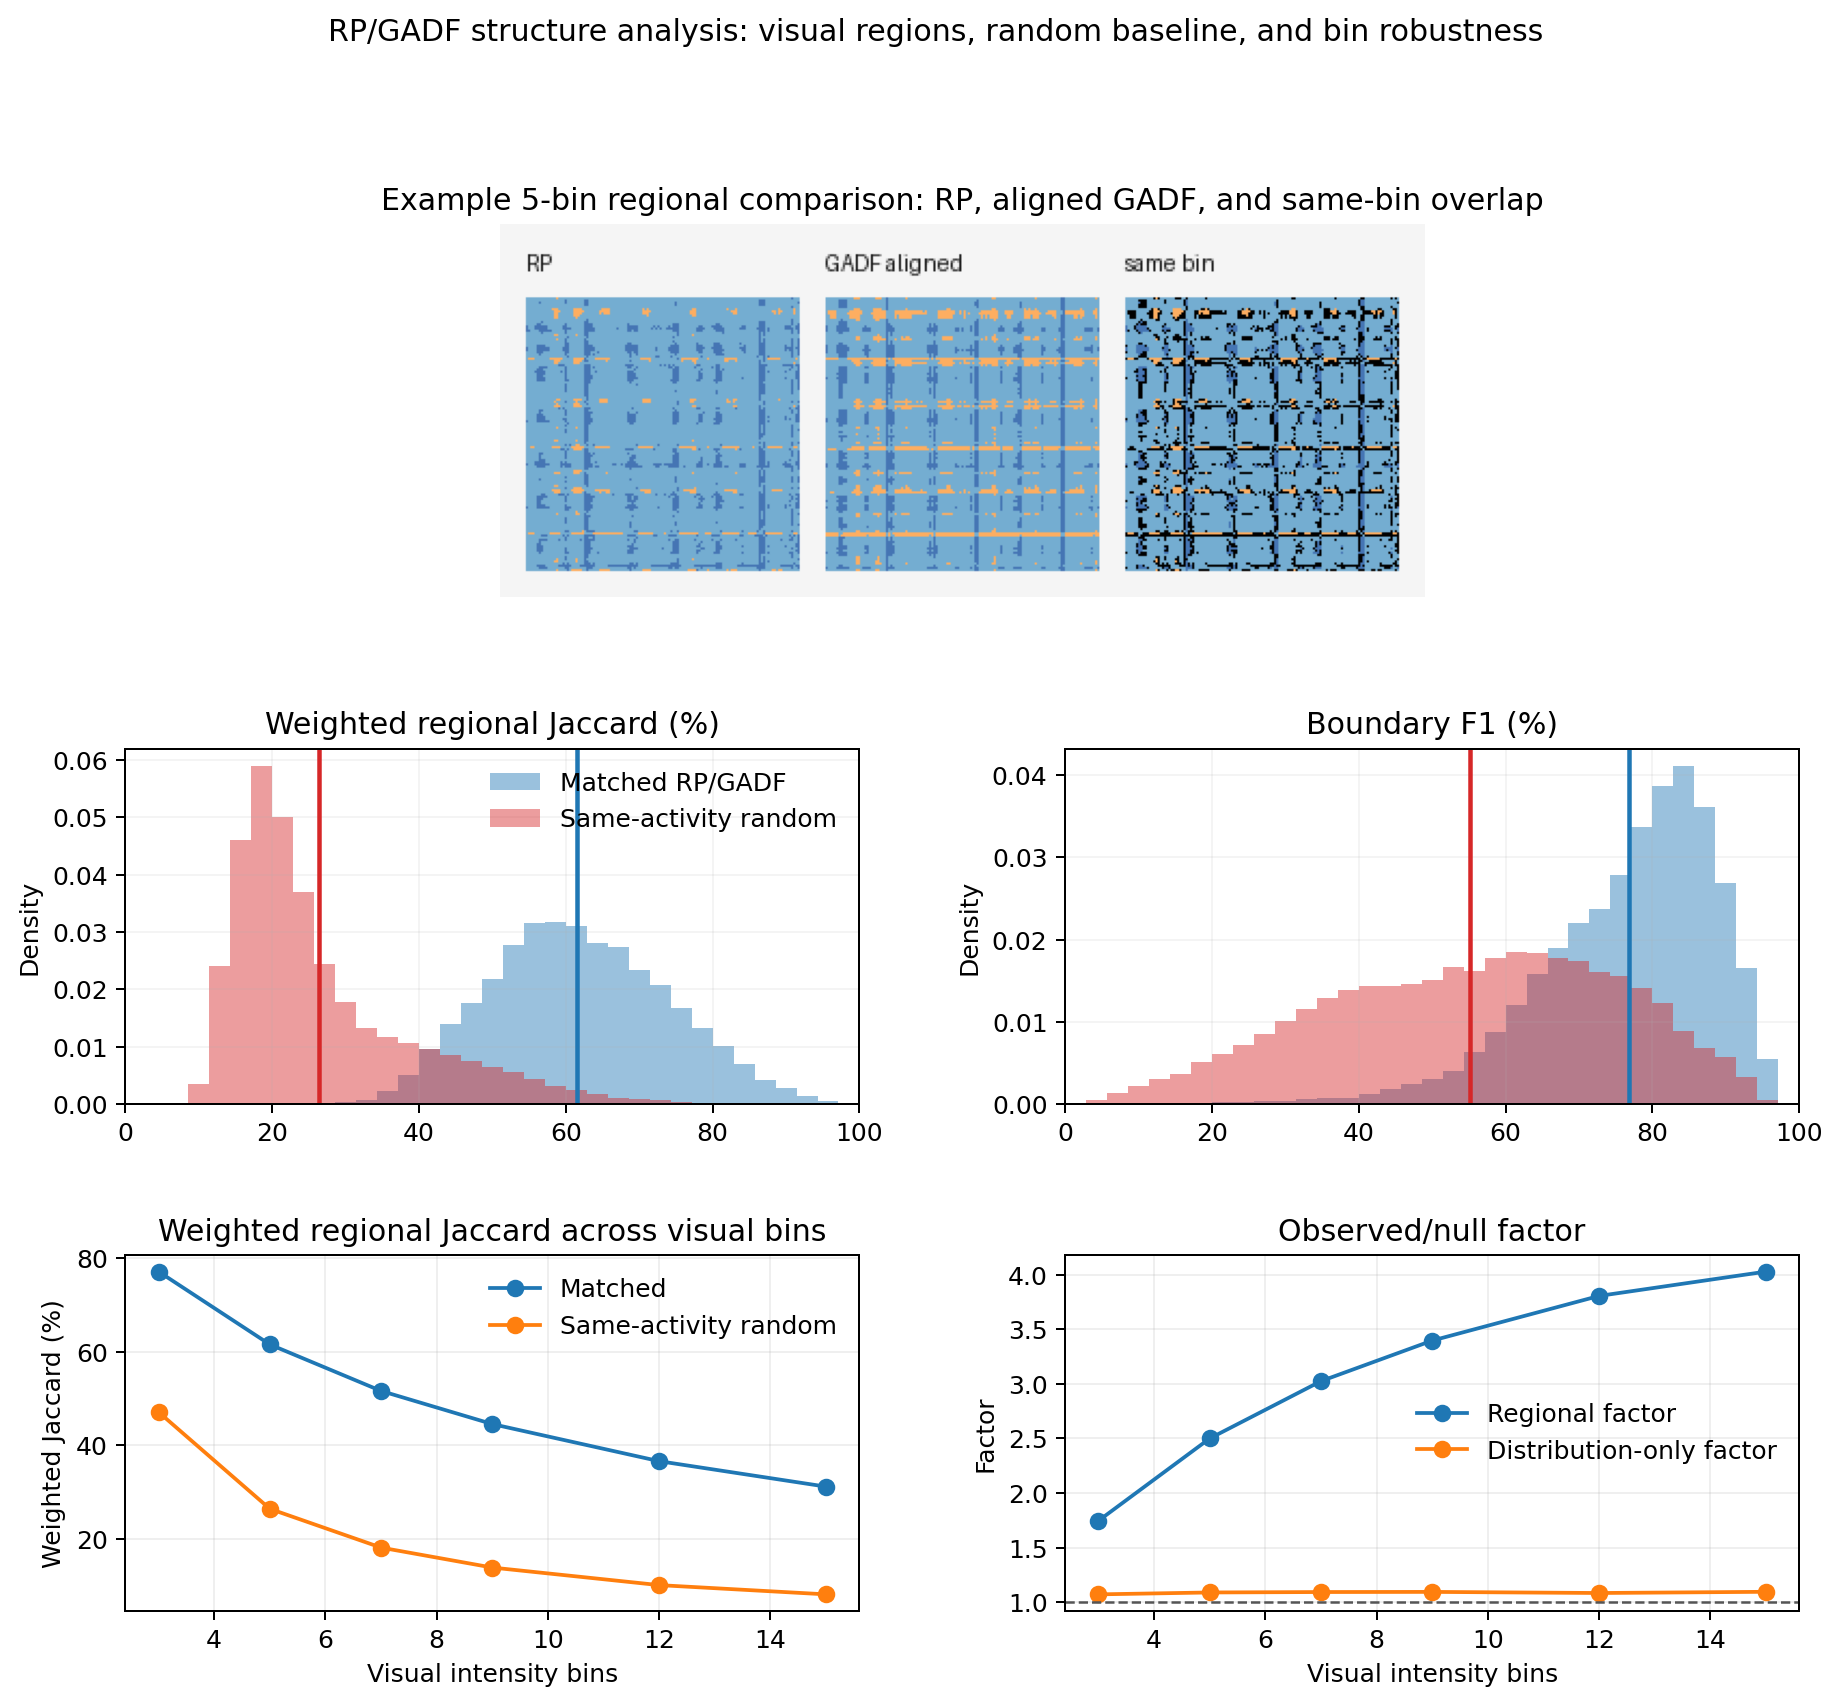
\includegraphics[width=0.92\textwidth]{images/rp_gadf_structure_collage.png}
    \caption{Null-corrected RP/GADF structural-overlap diagnostic. The top panel shows one 5-bin visual comparison: quantised RP, aligned quantised GADF, and pixels landing in the same bin. The middle histograms compare matched RP/GADF pairs against same-activity random pairings. The bottom row shows that matched regional overlap remains above the null baseline across independent visual quantisation levels \(B\in\{3,5,7,9,12,15\}\), while the distribution-only factor stays close to one.}
    \label{fig:rp_gadf_structure_overlap}
\end{figure}
\FloatBarrier

\begin{table}[H]
\centering
\caption{Null-corrected RP/GADF weighted regional overlap across visual intensity bins. Values are averaged over grayscale and the three axis channels. The null baseline pairs each RP image with a GADF image from a different window of the same activity class. Jaccard values are percentages; the Matched/null factor is the mean over the four channels of the per-channel matched/null ratio, so it is not the ratio of the two displayed column means.}
\label{tab:rp_gadf_region_overlap}
\setlength{\tabcolsep}{6pt}
\footnotesize
\begin{tabular}{@{}ccccc@{}}
\toprule
Visual bins \(B\) & Matched Jaccard & Same-activity null & Matched--null gain & Matched/null factor \\
\midrule
3  & 77.16 & 47.11 & +30.05 & \(1.75\times\) \\
5  & 61.57 & 26.43 & +35.14 & \(2.50\times\) \\
7  & 51.64 & 18.14 & +33.50 & \(3.02\times\) \\
9  & 44.55 & 13.87 & +30.68 & \(3.40\times\) \\
12 & 36.62 & 10.12 & +26.50 & \(3.81\times\) \\
15 & 31.17 & 8.14  & +23.03 & \(4.03\times\) \\
\bottomrule
\end{tabular}
\end{table}
\FloatBarrier

Table~\ref{tab:rp_gadf_region_overlap} and Figure~\ref{fig:rp_gadf_structure_overlap} support a narrow but useful claim: RP and GADF are not equivalent encodings, yet their coarse regions are substantially more aligned when they come from the same signal window than when activity label alone is controlled. As \(B\) increases, the absolute Jaccard necessarily decreases because the region match becomes stricter, but the matched/null factor rises from \(1.75\times\) to \(4.03\times\). This is exactly the pattern expected if the shared structure is spatial rather than a by-product of broad intensity histograms. The distribution-only factor stays near \(1.07\times\)--\(1.09\times\) across the same sweep, so marginal colour occupancy explains only a small part of the effect. Boundary F1 gives the same sign of evidence at coarse quantisation, but becomes less diagnostic at high \(B\) because every image develops many region edges; for that reason we treat weighted regional Jaccard as the primary overlap statistic.
\subsection{Structural relationship between signed RP and GADF}
\label{sec:supp_structural}
\paragraph*{Operator-level comparison of pairwise structure.}
Before discussing the first-order amplitude expansion that the rest of this section relies on, it is useful to put signed RP and GADF in a common notation without claiming equality of their output spaces. Both can be written as pairwise functions of lifted scalar samples,
\[
M_{ij} \;=\; \omega\!\bigl(\xi(x_i),\,\xi(x_j)\bigr),
\]
where $\xi:\mathbb{R}\to\mathbb{R}^{2}$ is a two-dimensional lift of the scalar sample and $\omega:\mathbb{R}^{2}\times\mathbb{R}^{2}\to\mathbb{R}$ is the pairwise operator associated with the encoding. The two methods differ in both the lift and the operator:
\begin{itemize}
  \item RP under the Lu--Tong convention uses the adjacent-state embedding \(\xi_{\text{RP}}(x_k)=(x_k,\,x_{k+1})\) and a signed Euclidean distance, \(\omega_{\text{RP}}(u,v)=\sigma(u,v)\lVert u-v\rVert_{2}\), where the sign is assigned \emph{externally} by the projection onto the reference direction \(v_{\star}=(1,1)^{\top}/\sqrt{2}\). With the thresholded sign rule used here, \(\sigma(u,v)\) is not guaranteed to satisfy \(\sigma(u,v)=-\sigma(v,u)\) for every pair, so the resulting matrix is directional but not necessarily antisymmetric.
  \item GADF uses the polar lift \(\xi_{\text{GADF}}(\tilde x_k)=(\tilde x_k,\sqrt{1-\tilde x_k^{2}})=(\cos\phi_k,\sin\phi_k)\) and the operator \(\omega_{\text{GADF}}(u,v)=\det[v\mid u]=u_{2}v_{1}-u_{1}v_{2}=\sin(\phi_i-\phi_j)\), the signed area of the parallelogram spanned by the two lifted points, whose sign is \emph{intrinsic} to the operator and matches \(G^{\mathrm{D}}_{ij}\) in Eq.~\eqref{eq:gadf_indexed}.
\end{itemize}
The important consequence is therefore an analogy, not an identity. GADF lies \emph{within} the $\binom{N}{2}$-dimensional space of antisymmetric zero-diagonal matrices by construction, because the determinant changes sign when its arguments are swapped; more specifically, its factorisation $G^{\mathrm{D}}=\mathbf{s}\,\mathbf{c}^{\top}-\mathbf{c}\,\mathbf{s}^{\top}$ (with $s_i=\sin\phi_i$, $c_i=\cos\phi_i$) shows it occupies only a rank-$\leq 2$ subvariety of that ambient space, not the whole of it. Signed RP has a zero diagonal and carries directional pairwise-distance information, but the Lu--Tong sign rule used in this paper does not force exact antisymmetry for nearly orthogonal displacements. The first-order expansion below quantifies why the two images can nevertheless look and behave similarly, while the structural differences between the two operators --- GADF's intrinsic sign and its closed-form one-pass inverse, versus signed RP's externally assigned sign and its MDS-based reconstruction --- follow from the determinant-based operator rather than from an exact shared matrix space.

\paragraph*{A structural reading of why RP and GADF look (and behave) so similarly.}
Beyond the empirical ranking, the proximity between RP and GADF deserves a structural reading: their visual resemblance and their adjacent positions in the evaluation ranking are not coincidental. GADF produces an antisymmetric zero-diagonal matrix, while signed RP produces a zero-diagonal directional distance matrix with related pairwise-difference content. For smooth signals whose local increments vary slowly (so that $x_{i+1}-x_i\approx x_{j+1}-x_j$ over the compared indices), both reduce, in first order, to functions of the pairwise-difference matrix $\{x_i-x_j\}_{i,j}$. The signed RP under the Lu--Tong embedding satisfies
\[
R_{ij} \;\approx\; \sigma(i,j)\,\sqrt{2}\,|x_i-x_j|,
\]
where $\sigma(i,j)$ is the external orientation flag computed from the projection of $s_i-s_j$ onto $v=(1,1)^\top/\sqrt{2}$. The GADF entry, expanded around a common normalized amplitude $\bar{x}$, satisfies
\[
G^{\mathrm{D}}_{ij} \;=\; \sin(\phi_i-\phi_j) \;\approx\; \frac{\bar{x}_j-\bar{x}_i}{\sqrt{1-\bar{x}^2}},
\]
because $d(\arccos x)/dx=-1/\sqrt{1-x^2}$, with both the samples $\bar{x}_i,\bar{x}_j$ and the expansion point $\bar{x}$ taken in the restricted $[-\alpha,\alpha]$ normalization of the GADF decoder. The sign of the GADF term is intrinsic to the trigonometric form rather than imposed externally. Thus, both expressions are linear in pairwise amplitude differences at first order and both are zero on the diagonal, but only GADF is strictly antisymmetric under the stated construction. What makes the restricted-branch GADF decoder closed-form is that it (i) makes the sign part of the encoding rather than a post-hoc convention, and (ii) restricts the angular range to $[\arccos(\alpha),\arccos(-\alpha)]$ with $\alpha=0.7$, a near-maximal symmetric choice below $1/\sqrt{2}$ that keeps every $\sin(\phi_i-\phi_j)$ inside the principal branch of $\arcsin$. In other words, GADF and signed RP are structurally adjacent parametrizations of directional pairwise differences: GADF makes the inverse map explicit in one closed-form pass under the branch restriction, while signed RP recovers the same directional structure through classical MDS with a signed-orientation step. This reading clarifies why GADF is the natural Gramian counterpart to signed RP --- the two are closer to each other than to either GASF or MTF, and both resolve the orientation ambiguity of the pairwise-difference representation, GADF intrinsically through $\sin$ and signed RP through its external sign convention.

\paragraph*{Practical implication: RP, GASF and GADF are three near-lossless inverses of a shared directional-difference structure.}
The structural analogy above has a direct consequence for interpretation. The visual resemblance between the RP and GADF images is not a coincidence of pixel statistics --- it follows from the first-order relations $R_{ij}\propto \sigma(i,j)|x_i-x_j|$ and $G^{\mathrm{D}}_{ij}\propto (\bar{x}_j-\bar{x}_i)/\sqrt{1-\bar{x}^2}$ derived above, and the null-corrected regional-overlap diagnostic of Section~\ref{sec:disc_rp_gadf_overlap} confirms that matched RP/GADF windows share more spatial region structure than same-activity random pairings. GASF encodes the symmetric, amplitude-bearing part of the Gramian (diagonal $\cos(2\phi_i)$); GADF encodes the antisymmetric, difference-bearing part ($\sin(\phi_i-\phi_j)$); signed RP encodes a directional distance structure with additional sensitivity to the local derivative through the $(x_i,x_{i+1})$ pair embedding. Our empirical numbers confirm this analytical picture: RP, GASF and GADF all invert near-losslessly and are statistically indistinguishable from the original on every classifier, so all three serve as reversible substrates for the controlled reconstruction problem studied here. GADF has the practical advantage of a closed-form, one-pass inverse through the determinant operator, whereas RP additionally exposes recurrence geometry and therefore remains the natural choice when recurrence quantification, dynamical invariants or line-structure statistics are themselves the object of study.

\appendix
\section{Per-Axis Reconstruction Errors}
\label{app:per_axis_errors}

Table~\ref{tab:pointwise_pooled} in the main text reports the per-window global reconstruction error (averaged over the three accelerometer axes) for each encoder. This appendix gives the per-axis breakdown over the same $N=8172$ pooled windows for RP (Table~\ref{tab:recurrence_plot}), MTF (Table~\ref{tab:markov_fields}), GASF (Table~\ref{tab:grammian_fields}) and GADF (Table~\ref{tab:gadf_fields}); in each, the Global column reproduces the per-window global figure of Table~\ref{tab:pointwise_pooled}.

\begin{table}[H]
\centering
\caption{RP per-axis reconstruction errors over all $N=8172$ pooled windows (physical units, m/s$^2$); mean$\pm$std across windows. The Global column averages the three axes per window.}
\label{tab:recurrence_plot}
\resizebox{\textwidth}{!}{%
\begin{tabular}{lcccc}
\toprule
\textbf{Metric} & \textbf{Dim 0} & \textbf{Dim 1} & \textbf{Dim 2} & \textbf{Global} \\
\midrule
Mean Absolute Error & $0.0148 \pm 0.0214$ & $0.0183 \pm 0.0264$ & $0.0114 \pm 0.0153$ & $0.0148 \pm 0.0170$ \\
Mean Squared Error & $0.0010 \pm 0.0076$ & $0.0015 \pm 0.0090$ & $0.0005 \pm 0.0027$ & $0.0010 \pm 0.0046$ \\
Pearson Correlation Coefficient & $0.99998 \pm 0.00009$ & $0.99998 \pm 0.00005$ & $0.99998 \pm 0.00006$ & $0.99998 \pm 0.00005$ \\
\bottomrule
\end{tabular}
}
\end{table}

\begin{table}[H]
\centering
\caption{MTF per-axis reconstruction errors over all $N=8172$ pooled windows (physical units, m/s$^2$); mean$\pm$std across windows. The Global column averages the three axes per window.}
\label{tab:markov_fields}
\resizebox{\textwidth}{!}{%
\begin{tabular}{lcccc}
\toprule
\textbf{Metric} & \textbf{Dim 0} & \textbf{Dim 1} & \textbf{Dim 2} & \textbf{Global} \\
\midrule
Mean Absolute Error & $4.13 \pm 5.11$ & $4.18 \pm 5.32$ & $3.53 \pm 4.66$ & $3.94 \pm 4.25$ \\
Mean Squared Error & $57.39 \pm 123.57$ & $61.72 \pm 157.60$ & $47.18 \pm 158.11$ & $55.43 \pm 113.46$ \\
Pearson Correlation Coefficient & $-0.00214 \pm 0.84525$ & $0.03600 \pm 0.83941$ & $0.00680 \pm 0.82844$ & $0.01356 \pm 0.48870$ \\
\bottomrule
\end{tabular}
}
\end{table}

\begin{table}[H]
\centering
\caption{GASF per-axis reconstruction errors over all $N=8172$ pooled windows (physical units, m/s$^2$); mean$\pm$std across windows. The Global column averages the three axes per window.}
\label{tab:grammian_fields}
\resizebox{\textwidth}{!}{%
\begin{tabular}{lcccc}
\toprule
\textbf{Metric} & \textbf{Dim 0} & \textbf{Dim 1} & \textbf{Dim 2} & \textbf{Global} \\
\midrule
Mean Absolute Error & $0.0236 \pm 0.0243$ & $0.0195 \pm 0.0223$ & $0.0183 \pm 0.0216$ & $0.0205 \pm 0.0199$ \\
Mean Squared Error & $0.0050 \pm 0.0107$ & $0.0048 \pm 0.0127$ & $0.0030 \pm 0.0121$ & $0.0043 \pm 0.0088$ \\
Pearson Correlation Coefficient & $0.99987 \pm 0.00020$ & $0.99990 \pm 0.00024$ & $0.99987 \pm 0.00027$ & $0.99988 \pm 0.00014$ \\
\bottomrule
\end{tabular}
}
\end{table}

\begin{table}[H]
\centering
\caption{GADF per-axis reconstruction errors over all $N=8172$ pooled windows (physical units, m/s$^2$); mean$\pm$std across windows. The Global column averages the three axes per window.}
\label{tab:gadf_fields}
\resizebox{\textwidth}{!}{%
\begin{tabular}{lcccc}
\toprule
\textbf{Metric} & \textbf{Dim 0} & \textbf{Dim 1} & \textbf{Dim 2} & \textbf{Global} \\
\midrule
Mean Absolute Error & $0.0159 \pm 0.0189$ & $0.0169 \pm 0.0215$ & $0.0144 \pm 0.0199$ & $0.0157 \pm 0.0167$ \\
Mean Squared Error & $0.0008 \pm 0.0020$ & $0.0009 \pm 0.0028$ & $0.0007 \pm 0.0028$ & $0.0008 \pm 0.0018$ \\
Pearson Correlation Coefficient & $0.99999 \pm 0.00002$ & $0.99999 \pm 0.00002$ & $0.99999 \pm 0.00002$ & $0.99999 \pm 0.00001$ \\
\bottomrule
\end{tabular}
}
\end{table}

\FloatBarrier

\section{Per-Class Classification Results}
\label{app:per_class_results}

This appendix reports the complete per-class precision, recall, and
F1-score results for the six evaluated classifiers. The main text
retains only the compact accuracy comparison required to interpret
the differences among reconstruction methods. Per-class Support values are per-class fold-means rounded to integers and may sum to $2723$ rather than the $2724$ windows per fold reported in the Accuracy row (independent rounding).

\FloatBarrier
\begin{landscape}

\begin{table}[H]
\centering
\caption{Classification Results for GRU on the stratified window-level 3-fold protocol (mean $\pm$ std across folds 0, 1, 2). Per-class precision/recall/F1 and support averaged over the same three folds; footer accuracies averaged likewise.}
\label{tab:gru_classifiers}
\setlength{\tabcolsep}{2pt}
\resizebox{\linewidth}{!}{%
\begin{tabular}{l|cccc|cccc|cccc|cccc|cccc}
\toprule
          & \multicolumn{4}{c|}{Original} & \multicolumn{4}{c|}{RP} & \multicolumn{4}{c|}{MTF} & \multicolumn{4}{c|}{GASF} & \multicolumn{4}{c}{GADF} \\
\cmidrule(lr){2-5}\cmidrule(lr){6-9}\cmidrule(lr){10-13}\cmidrule(lr){14-17}\cmidrule(lr){18-21}
Class & Prec & Rec & F1 & Supp & Prec & Rec & F1 & Supp & Prec & Rec & F1 & Supp & Prec & Rec & F1 & Supp & Prec & Rec & F1 & Supp \\
\midrule
0 & 0.89$\pm$0.03 & 0.93$\pm$0.01 & 0.91$\pm$0.01 & 544 & 0.89$\pm$0.03 & 0.93$\pm$0.01 & 0.91$\pm$0.01 & 544 & 0.65$\pm$0.01 & 0.61$\pm$0.04 & 0.63$\pm$0.01 & 544 & 0.89$\pm$0.03 & 0.93$\pm$0.01 & 0.91$\pm$0.01 & 544 & 0.89$\pm$0.03 & 0.93$\pm$0.01 & 0.91$\pm$0.01 & 544 \\
1 & 0.99$\pm$0.01 & 0.99$\pm$0.00 & 0.99$\pm$0.00 & 532 & 0.99$\pm$0.01 & 0.99$\pm$0.00 & 0.99$\pm$0.00 & 532 & 0.75$\pm$0.02 & 0.99$\pm$0.00 & 0.85$\pm$0.01 & 532 & 0.99$\pm$0.01 & 0.99$\pm$0.00 & 0.99$\pm$0.00 & 532 & 0.99$\pm$0.01 & 0.99$\pm$0.00 & 0.99$\pm$0.00 & 532 \\
2 & 0.91$\pm$0.01 & 0.86$\pm$0.03 & 0.88$\pm$0.01 & 536 & 0.91$\pm$0.01 & 0.86$\pm$0.03 & 0.88$\pm$0.01 & 536 & 0.57$\pm$0.01 & 0.52$\pm$0.03 & 0.54$\pm$0.01 & 536 & 0.91$\pm$0.01 & 0.86$\pm$0.03 & 0.88$\pm$0.01 & 536 & 0.91$\pm$0.01 & 0.86$\pm$0.03 & 0.88$\pm$0.01 & 536 \\
3 & 0.88$\pm$0.01 & 0.96$\pm$0.01 & 0.92$\pm$0.00 & 551 & 0.88$\pm$0.01 & 0.96$\pm$0.01 & 0.92$\pm$0.00 & 551 & 0.90$\pm$0.01 & 0.90$\pm$0.01 & 0.90$\pm$0.01 & 551 & 0.88$\pm$0.01 & 0.96$\pm$0.01 & 0.92$\pm$0.00 & 551 & 0.88$\pm$0.01 & 0.96$\pm$0.01 & 0.92$\pm$0.00 & 551 \\
4 & 0.95$\pm$0.01 & 0.89$\pm$0.01 & 0.92$\pm$0.00 & 560 & 0.95$\pm$0.01 & 0.89$\pm$0.01 & 0.92$\pm$0.00 & 560 & 0.96$\pm$0.01 & 0.81$\pm$0.01 & 0.88$\pm$0.00 & 560 & 0.95$\pm$0.01 & 0.89$\pm$0.01 & 0.92$\pm$0.00 & 560 & 0.95$\pm$0.01 & 0.89$\pm$0.01 & 0.92$\pm$0.00 & 560 \\
\midrule
Accuracy & \multicolumn{4}{c|}{0.92$\pm$0.00 (2724)} & \multicolumn{4}{c|}{0.92$\pm$0.00 (2724)} & \multicolumn{4}{c|}{0.77$\pm$0.01 (2724)} & \multicolumn{4}{c|}{0.92$\pm$0.00 (2724)} & \multicolumn{4}{c}{0.92$\pm$0.00 (2724)} \\
Macro Avg & \multicolumn{4}{c|}{0.93$\pm$0.00/0.92$\pm$0.00/0.92$\pm$0.00} & \multicolumn{4}{c|}{0.92$\pm$0.00/0.92$\pm$0.00/0.92$\pm$0.00} & \multicolumn{4}{c|}{0.77$\pm$0.01/0.76$\pm$0.01/0.76$\pm$0.01} & \multicolumn{4}{c|}{0.92$\pm$0.00/0.92$\pm$0.00/0.92$\pm$0.00} & \multicolumn{4}{c}{0.93$\pm$0.00/0.92$\pm$0.00/0.92$\pm$0.00} \\
Weighted Avg & \multicolumn{4}{c|}{0.93$\pm$0.00/0.92$\pm$0.00/0.92$\pm$0.00} & \multicolumn{4}{c|}{0.92$\pm$0.00/0.92$\pm$0.00/0.92$\pm$0.00} & \multicolumn{4}{c|}{0.77$\pm$0.01/0.77$\pm$0.01/0.76$\pm$0.01} & \multicolumn{4}{c|}{0.92$\pm$0.00/0.92$\pm$0.00/0.92$\pm$0.00} & \multicolumn{4}{c}{0.93$\pm$0.00/0.92$\pm$0.00/0.92$\pm$0.00} \\


\bottomrule
\end{tabular}}
\end{table}

\begin{table}[H]
\centering
\caption{Classification Results for KNN on the stratified window-level 3-fold protocol (mean $\pm$ std across folds 0, 1, 2). Per-class precision/recall/F1 and support averaged over the same three folds; footer accuracies averaged likewise.}
\label{tab:knn_classifiers}
\setlength{\tabcolsep}{2pt}
\resizebox{\linewidth}{!}{%
\begin{tabular}{l|cccc|cccc|cccc|cccc|cccc}
\toprule
          & \multicolumn{4}{c|}{Original} & \multicolumn{4}{c|}{RP} & \multicolumn{4}{c|}{MTF} & \multicolumn{4}{c|}{GASF} & \multicolumn{4}{c}{GADF} \\
\cmidrule(lr){2-5}\cmidrule(lr){6-9}\cmidrule(lr){10-13}\cmidrule(lr){14-17}\cmidrule(lr){18-21}
Class & Prec & Rec & F1 & Supp & Prec & Rec & F1 & Supp & Prec & Rec & F1 & Supp & Prec & Rec & F1 & Supp & Prec & Rec & F1 & Supp \\
\midrule
0 & 0.74$\pm$0.01 & 0.52$\pm$0.01 & 0.61$\pm$0.01 & 544 & 0.74$\pm$0.01 & 0.52$\pm$0.01 & 0.61$\pm$0.01 & 544 & 0.64$\pm$0.01 & 0.49$\pm$0.02 & 0.55$\pm$0.01 & 544 & 0.74$\pm$0.01 & 0.52$\pm$0.01 & 0.61$\pm$0.01 & 544 & 0.74$\pm$0.01 & 0.52$\pm$0.01 & 0.61$\pm$0.01 & 544 \\
1 & 1.00$\pm$0.00 & 0.75$\pm$0.01 & 0.86$\pm$0.01 & 532 & 1.00$\pm$0.00 & 0.75$\pm$0.01 & 0.86$\pm$0.01 & 532 & 0.99$\pm$0.02 & 0.37$\pm$0.00 & 0.54$\pm$0.00 & 532 & 1.00$\pm$0.00 & 0.75$\pm$0.01 & 0.86$\pm$0.01 & 532 & 1.00$\pm$0.00 & 0.75$\pm$0.01 & 0.86$\pm$0.01 & 532 \\
2 & 0.49$\pm$0.04 & 0.04$\pm$0.01 & 0.08$\pm$0.02 & 536 & 0.49$\pm$0.04 & 0.04$\pm$0.01 & 0.08$\pm$0.01 & 536 & 0.43$\pm$0.04 & 0.07$\pm$0.00 & 0.12$\pm$0.00 & 536 & 0.50$\pm$0.04 & 0.04$\pm$0.01 & 0.08$\pm$0.02 & 536 & 0.50$\pm$0.04 & 0.04$\pm$0.01 & 0.08$\pm$0.01 & 536 \\
3 & 0.79$\pm$0.00 & 0.96$\pm$0.00 & 0.87$\pm$0.00 & 551 & 0.79$\pm$0.00 & 0.96$\pm$0.00 & 0.87$\pm$0.00 & 551 & 0.63$\pm$0.01 & 0.94$\pm$0.01 & 0.75$\pm$0.01 & 551 & 0.79$\pm$0.00 & 0.96$\pm$0.00 & 0.87$\pm$0.00 & 551 & 0.79$\pm$0.00 & 0.96$\pm$0.00 & 0.87$\pm$0.00 & 551 \\
4 & 0.42$\pm$0.00 & 0.92$\pm$0.01 & 0.58$\pm$0.00 & 560 & 0.42$\pm$0.00 & 0.92$\pm$0.01 & 0.58$\pm$0.00 & 560 & 0.42$\pm$0.01 & 0.90$\pm$0.01 & 0.57$\pm$0.01 & 560 & 0.42$\pm$0.00 & 0.92$\pm$0.01 & 0.58$\pm$0.00 & 560 & 0.42$\pm$0.00 & 0.92$\pm$0.01 & 0.58$\pm$0.00 & 560 \\
\midrule
Accuracy & \multicolumn{4}{c|}{0.64$\pm$0.00 (2724)} & \multicolumn{4}{c|}{0.64$\pm$0.00 (2724)} & \multicolumn{4}{c|}{0.56$\pm$0.01 (2724)} & \multicolumn{4}{c|}{0.64$\pm$0.00 (2724)} & \multicolumn{4}{c}{0.64$\pm$0.00 (2724)} \\
Macro Avg & \multicolumn{4}{c|}{0.69$\pm$0.01/0.64$\pm$0.00/0.60$\pm$0.00} & \multicolumn{4}{c|}{0.69$\pm$0.01/0.64$\pm$0.00/0.60$\pm$0.00} & \multicolumn{4}{c|}{0.62$\pm$0.01/0.55$\pm$0.01/0.51$\pm$0.01} & \multicolumn{4}{c|}{0.69$\pm$0.01/0.64$\pm$0.00/0.60$\pm$0.00} & \multicolumn{4}{c}{0.69$\pm$0.01/0.64$\pm$0.00/0.60$\pm$0.00} \\
Weighted Avg & \multicolumn{4}{c|}{0.69$\pm$0.01/0.64$\pm$0.00/0.60$\pm$0.00} & \multicolumn{4}{c|}{0.69$\pm$0.01/0.64$\pm$0.00/0.60$\pm$0.00} & \multicolumn{4}{c|}{0.62$\pm$0.01/0.56$\pm$0.01/0.51$\pm$0.01} & \multicolumn{4}{c|}{0.69$\pm$0.01/0.64$\pm$0.00/0.60$\pm$0.00} & \multicolumn{4}{c}{0.69$\pm$0.01/0.64$\pm$0.00/0.60$\pm$0.00} \\


\bottomrule
\end{tabular}}
\end{table}

\begin{table}[H]
\centering
\caption{Classification Results for CNN on the stratified window-level 3-fold protocol (mean $\pm$ std across folds 0, 1, 2). Per-class precision/recall/F1 and support averaged over the same three folds; footer accuracies averaged likewise.}
\label{tab:cnn_classifiers}
\setlength{\tabcolsep}{2pt}
\resizebox{\linewidth}{!}{%
\begin{tabular}{l|cccc|cccc|cccc|cccc|cccc}
\toprule
          & \multicolumn{4}{c|}{Original} & \multicolumn{4}{c|}{RP} & \multicolumn{4}{c|}{MTF} & \multicolumn{4}{c|}{GASF} & \multicolumn{4}{c}{GADF} \\
\cmidrule(lr){2-5}\cmidrule(lr){6-9}\cmidrule(lr){10-13}\cmidrule(lr){14-17}\cmidrule(lr){18-21}
Class & Prec & Rec & F1 & Supp & Prec & Rec & F1 & Supp & Prec & Rec & F1 & Supp & Prec & Rec & F1 & Supp & Prec & Rec & F1 & Supp \\
\midrule
0 & 0.89$\pm$0.05 & 0.89$\pm$0.05 & 0.89$\pm$0.01 & 544 & 0.91$\pm$0.02 & 0.85$\pm$0.05 & 0.87$\pm$0.02 & 544 & 0.61$\pm$0.07 & 0.73$\pm$0.08 & 0.66$\pm$0.01 & 544 & 0.89$\pm$0.05 & 0.89$\pm$0.05 & 0.89$\pm$0.01 & 544 & 0.89$\pm$0.05 & 0.89$\pm$0.05 & 0.89$\pm$0.01 & 544 \\
1 & 0.99$\pm$0.01 & 0.98$\pm$0.00 & 0.99$\pm$0.00 & 532 & 0.98$\pm$0.01 & 0.99$\pm$0.00 & 0.99$\pm$0.00 & 532 & 0.88$\pm$0.03 & 0.97$\pm$0.02 & 0.92$\pm$0.01 & 532 & 0.99$\pm$0.01 & 0.98$\pm$0.00 & 0.99$\pm$0.00 & 532 & 0.99$\pm$0.01 & 0.98$\pm$0.00 & 0.99$\pm$0.00 & 532 \\
2 & 0.88$\pm$0.04 & 0.87$\pm$0.05 & 0.87$\pm$0.01 & 536 & 0.84$\pm$0.04 & 0.90$\pm$0.03 & 0.86$\pm$0.01 & 536 & 0.62$\pm$0.03 & 0.55$\pm$0.10 & 0.57$\pm$0.05 & 536 & 0.88$\pm$0.04 & 0.87$\pm$0.05 & 0.87$\pm$0.01 & 536 & 0.88$\pm$0.04 & 0.87$\pm$0.05 & 0.87$\pm$0.01 & 536 \\
3 & 0.84$\pm$0.05 & 0.97$\pm$0.02 & 0.90$\pm$0.02 & 551 & 0.84$\pm$0.03 & 0.97$\pm$0.01 & 0.90$\pm$0.01 & 551 & 0.85$\pm$0.04 & 0.89$\pm$0.04 & 0.87$\pm$0.01 & 551 & 0.84$\pm$0.04 & 0.97$\pm$0.02 & 0.90$\pm$0.02 & 551 & 0.84$\pm$0.05 & 0.97$\pm$0.02 & 0.90$\pm$0.02 & 551 \\
4 & 0.97$\pm$0.02 & 0.83$\pm$0.05 & 0.89$\pm$0.02 & 560 & 0.98$\pm$0.00 & 0.81$\pm$0.02 & 0.88$\pm$0.01 & 560 & 0.97$\pm$0.03 & 0.73$\pm$0.04 & 0.83$\pm$0.02 & 560 & 0.97$\pm$0.02 & 0.83$\pm$0.05 & 0.89$\pm$0.02 & 560 & 0.97$\pm$0.02 & 0.82$\pm$0.05 & 0.89$\pm$0.02 & 560 \\
\midrule
Accuracy & \multicolumn{4}{c|}{0.91$\pm$0.00 (2724)} & \multicolumn{4}{c|}{0.90$\pm$0.01 (2724)} & \multicolumn{4}{c|}{0.77$\pm$0.01 (2724)} & \multicolumn{4}{c|}{0.91$\pm$0.01 (2724)} & \multicolumn{4}{c}{0.91$\pm$0.00 (2724)} \\
Macro Avg & \multicolumn{4}{c|}{0.91$\pm$0.00/0.91$\pm$0.00/0.91$\pm$0.00} & \multicolumn{4}{c|}{0.91$\pm$0.00/0.90$\pm$0.01/0.90$\pm$0.01} & \multicolumn{4}{c|}{0.79$\pm$0.01/0.77$\pm$0.01/0.77$\pm$0.01} & \multicolumn{4}{c|}{0.91$\pm$0.00/0.91$\pm$0.01/0.91$\pm$0.01} & \multicolumn{4}{c}{0.91$\pm$0.00/0.91$\pm$0.00/0.91$\pm$0.00} \\
Weighted Avg & \multicolumn{4}{c|}{0.91$\pm$0.00/0.91$\pm$0.00/0.91$\pm$0.01} & \multicolumn{4}{c|}{0.91$\pm$0.00/0.90$\pm$0.01/0.90$\pm$0.01} & \multicolumn{4}{c|}{0.79$\pm$0.01/0.77$\pm$0.01/0.77$\pm$0.01} & \multicolumn{4}{c|}{0.91$\pm$0.00/0.91$\pm$0.01/0.91$\pm$0.01} & \multicolumn{4}{c}{0.91$\pm$0.00/0.91$\pm$0.00/0.91$\pm$0.00} \\


\bottomrule
\end{tabular}}
\end{table}

\begin{table}[H]
\centering
\caption{Classification Results for Random Forest on the stratified window-level 3-fold protocol (mean $\pm$ std across folds 0, 1, 2). Per-class precision/recall/F1 and support averaged over the same three folds; footer accuracies averaged likewise.}
\label{tab:rf_classifiers}
\setlength{\tabcolsep}{2pt}
\resizebox{\linewidth}{!}{%
\begin{tabular}{l|cccc|cccc|cccc|cccc|cccc}
\toprule
          & \multicolumn{4}{c|}{Original} & \multicolumn{4}{c|}{RP} & \multicolumn{4}{c|}{MTF} & \multicolumn{4}{c|}{GASF} & \multicolumn{4}{c}{GADF} \\
\cmidrule(lr){2-5}\cmidrule(lr){6-9}\cmidrule(lr){10-13}\cmidrule(lr){14-17}\cmidrule(lr){18-21}
Class & Prec & Rec & F1 & Supp & Prec & Rec & F1 & Supp & Prec & Rec & F1 & Supp & Prec & Rec & F1 & Supp & Prec & Rec & F1 & Supp \\
\midrule
0 & 0.85$\pm$0.01 & 0.79$\pm$0.00 & 0.82$\pm$0.00 & 544 & 0.86$\pm$0.01 & 0.79$\pm$0.00 & 0.82$\pm$0.00 & 544 & 0.68$\pm$0.01 & 0.60$\pm$0.01 & 0.64$\pm$0.00 & 544 & 0.85$\pm$0.01 & 0.79$\pm$0.01 & 0.82$\pm$0.01 & 544 & 0.85$\pm$0.01 & 0.79$\pm$0.00 & 0.82$\pm$0.00 & 544 \\
1 & 0.94$\pm$0.00 & 0.99$\pm$0.00 & 0.96$\pm$0.00 & 532 & 0.94$\pm$0.00 & 0.99$\pm$0.00 & 0.96$\pm$0.00 & 532 & 0.65$\pm$0.01 & 1.00$\pm$0.00 & 0.79$\pm$0.01 & 532 & 0.94$\pm$0.00 & 0.99$\pm$0.00 & 0.96$\pm$0.00 & 532 & 0.94$\pm$0.00 & 0.99$\pm$0.00 & 0.96$\pm$0.00 & 532 \\
2 & 0.79$\pm$0.00 & 0.82$\pm$0.01 & 0.81$\pm$0.01 & 536 & 0.79$\pm$0.00 & 0.83$\pm$0.01 & 0.81$\pm$0.01 & 536 & 0.63$\pm$0.01 & 0.51$\pm$0.02 & 0.56$\pm$0.01 & 536 & 0.79$\pm$0.01 & 0.82$\pm$0.01 & 0.80$\pm$0.01 & 536 & 0.79$\pm$0.00 & 0.82$\pm$0.01 & 0.80$\pm$0.01 & 536 \\
3 & 0.92$\pm$0.01 & 0.95$\pm$0.00 & 0.93$\pm$0.01 & 551 & 0.92$\pm$0.01 & 0.95$\pm$0.00 & 0.93$\pm$0.01 & 551 & 0.93$\pm$0.01 & 0.89$\pm$0.01 & 0.91$\pm$0.00 & 551 & 0.92$\pm$0.01 & 0.95$\pm$0.00 & 0.93$\pm$0.01 & 551 & 0.92$\pm$0.01 & 0.95$\pm$0.00 & 0.93$\pm$0.00 & 551 \\
4 & 0.96$\pm$0.00 & 0.90$\pm$0.01 & 0.93$\pm$0.00 & 560 & 0.96$\pm$0.00 & 0.90$\pm$0.01 & 0.93$\pm$0.00 & 560 & 0.94$\pm$0.01 & 0.79$\pm$0.01 & 0.86$\pm$0.01 & 560 & 0.96$\pm$0.00 & 0.90$\pm$0.01 & 0.93$\pm$0.00 & 560 & 0.96$\pm$0.00 & 0.90$\pm$0.01 & 0.93$\pm$0.00 & 560 \\
\midrule
Accuracy & \multicolumn{4}{c|}{0.89$\pm$0.00 (2724)} & \multicolumn{4}{c|}{0.89$\pm$0.00 (2724)} & \multicolumn{4}{c|}{0.76$\pm$0.00 (2724)} & \multicolumn{4}{c|}{0.89$\pm$0.00 (2724)} & \multicolumn{4}{c}{0.89$\pm$0.00 (2724)} \\
Macro Avg & \multicolumn{4}{c|}{0.89$\pm$0.00/0.89$\pm$0.00/0.89$\pm$0.00} & \multicolumn{4}{c|}{0.89$\pm$0.00/0.89$\pm$0.00/0.89$\pm$0.00} & \multicolumn{4}{c|}{0.77$\pm$0.00/0.76$\pm$0.00/0.75$\pm$0.00} & \multicolumn{4}{c|}{0.89$\pm$0.00/0.89$\pm$0.00/0.89$\pm$0.00} & \multicolumn{4}{c}{0.89$\pm$0.00/0.89$\pm$0.00/0.89$\pm$0.00} \\
Weighted Avg & \multicolumn{4}{c|}{0.89$\pm$0.00/0.89$\pm$0.00/0.89$\pm$0.00} & \multicolumn{4}{c|}{0.89$\pm$0.00/0.89$\pm$0.00/0.89$\pm$0.00} & \multicolumn{4}{c|}{0.77$\pm$0.00/0.76$\pm$0.00/0.75$\pm$0.00} & \multicolumn{4}{c|}{0.89$\pm$0.00/0.89$\pm$0.00/0.89$\pm$0.00} & \multicolumn{4}{c}{0.89$\pm$0.00/0.89$\pm$0.00/0.89$\pm$0.00} \\


\bottomrule
\end{tabular}}
\end{table}

\begin{table}[H]
\centering
\caption{Classification Results for Support Vector Machine on the stratified window-level 3-fold protocol (mean $\pm$ std across folds 0, 1, 2). Per-class precision/recall/F1 and support averaged over the same three folds; footer accuracies averaged likewise.}
\label{tab:svm_classifiers}
\setlength{\tabcolsep}{2pt}
\resizebox{\linewidth}{!}{%
\begin{tabular}{l|cccc|cccc|cccc|cccc|cccc}
\toprule
          & \multicolumn{4}{c|}{Original} & \multicolumn{4}{c|}{RP} & \multicolumn{4}{c|}{MTF} & \multicolumn{4}{c|}{GASF} & \multicolumn{4}{c}{GADF} \\
\cmidrule(lr){2-5}\cmidrule(lr){6-9}\cmidrule(lr){10-13}\cmidrule(lr){14-17}\cmidrule(lr){18-21}
Class & Prec & Rec & F1 & Supp & Prec & Rec & F1 & Supp & Prec & Rec & F1 & Supp & Prec & Rec & F1 & Supp & Prec & Rec & F1 & Supp \\
\midrule
0 & 0.76$\pm$0.01 & 0.65$\pm$0.02 & 0.70$\pm$0.01 & 544 & 0.76$\pm$0.01 & 0.65$\pm$0.01 & 0.70$\pm$0.01 & 544 & 0.52$\pm$0.01 & 0.71$\pm$0.02 & 0.60$\pm$0.01 & 544 & 0.76$\pm$0.01 & 0.65$\pm$0.01 & 0.70$\pm$0.01 & 544 & 0.76$\pm$0.00 & 0.65$\pm$0.01 & 0.70$\pm$0.01 & 544 \\
1 & 0.97$\pm$0.01 & 0.97$\pm$0.00 & 0.97$\pm$0.00 & 532 & 0.97$\pm$0.01 & 0.97$\pm$0.00 & 0.97$\pm$0.00 & 532 & 0.69$\pm$0.01 & 1.00$\pm$0.00 & 0.81$\pm$0.01 & 532 & 0.97$\pm$0.01 & 0.97$\pm$0.00 & 0.97$\pm$0.00 & 532 & 0.97$\pm$0.01 & 0.97$\pm$0.00 & 0.97$\pm$0.00 & 532 \\
2 & 0.66$\pm$0.01 & 0.69$\pm$0.01 & 0.67$\pm$0.01 & 536 & 0.66$\pm$0.01 & 0.69$\pm$0.01 & 0.67$\pm$0.01 & 536 & 0.49$\pm$0.04 & 0.17$\pm$0.01 & 0.25$\pm$0.02 & 536 & 0.65$\pm$0.01 & 0.69$\pm$0.01 & 0.67$\pm$0.01 & 536 & 0.66$\pm$0.01 & 0.69$\pm$0.01 & 0.67$\pm$0.01 & 536 \\
3 & 0.84$\pm$0.01 & 0.84$\pm$0.00 & 0.84$\pm$0.00 & 551 & 0.84$\pm$0.01 & 0.84$\pm$0.00 & 0.84$\pm$0.00 & 551 & 0.86$\pm$0.01 & 0.81$\pm$0.01 & 0.83$\pm$0.00 & 551 & 0.84$\pm$0.01 & 0.84$\pm$0.00 & 0.84$\pm$0.00 & 551 & 0.84$\pm$0.01 & 0.84$\pm$0.00 & 0.84$\pm$0.00 & 551 \\
4 & 0.78$\pm$0.01 & 0.85$\pm$0.01 & 0.81$\pm$0.00 & 560 & 0.78$\pm$0.01 & 0.85$\pm$0.01 & 0.81$\pm$0.01 & 560 & 0.86$\pm$0.00 & 0.81$\pm$0.00 & 0.83$\pm$0.00 & 560 & 0.78$\pm$0.01 & 0.85$\pm$0.01 & 0.81$\pm$0.00 & 560 & 0.78$\pm$0.00 & 0.85$\pm$0.01 & 0.81$\pm$0.00 & 560 \\
\midrule
Accuracy & \multicolumn{4}{c|}{0.80$\pm$0.00 (2724)} & \multicolumn{4}{c|}{0.80$\pm$0.00 (2724)} & \multicolumn{4}{c|}{0.70$\pm$0.01 (2724)} & \multicolumn{4}{c|}{0.80$\pm$0.00 (2724)} & \multicolumn{4}{c}{0.80$\pm$0.00 (2724)} \\
Macro Avg & \multicolumn{4}{c|}{0.80$\pm$0.01/0.80$\pm$0.00/0.80$\pm$0.01} & \multicolumn{4}{c|}{0.80$\pm$0.01/0.80$\pm$0.00/0.80$\pm$0.00} & \multicolumn{4}{c|}{0.69$\pm$0.01/0.70$\pm$0.01/0.67$\pm$0.01} & \multicolumn{4}{c|}{0.80$\pm$0.01/0.80$\pm$0.00/0.80$\pm$0.01} & \multicolumn{4}{c}{0.80$\pm$0.00/0.80$\pm$0.00/0.80$\pm$0.00} \\
Weighted Avg & \multicolumn{4}{c|}{0.80$\pm$0.01/0.80$\pm$0.00/0.80$\pm$0.01} & \multicolumn{4}{c|}{0.80$\pm$0.01/0.80$\pm$0.00/0.80$\pm$0.00} & \multicolumn{4}{c|}{0.69$\pm$0.01/0.70$\pm$0.01/0.67$\pm$0.01} & \multicolumn{4}{c|}{0.80$\pm$0.01/0.80$\pm$0.00/0.80$\pm$0.01} & \multicolumn{4}{c}{0.80$\pm$0.00/0.80$\pm$0.00/0.80$\pm$0.00} \\


\bottomrule
\end{tabular}}
\end{table}

\begin{table}[H]
\centering
\caption{Classification Results for LSTM on the stratified window-level 3-fold protocol (mean $\pm$ std across folds 0, 1, 2). Per-class precision/recall/F1 and support averaged over the same three folds; footer accuracies averaged likewise.}
\label{tab:lstm_classifiers}
\setlength{\tabcolsep}{2pt}
\resizebox{\linewidth}{!}{%
\begin{tabular}{l|cccc|cccc|cccc|cccc|cccc}
\toprule
          & \multicolumn{4}{c|}{Original} & \multicolumn{4}{c|}{RP} & \multicolumn{4}{c|}{MTF} & \multicolumn{4}{c|}{GASF} & \multicolumn{4}{c}{GADF} \\
\cmidrule(lr){2-5}\cmidrule(lr){6-9}\cmidrule(lr){10-13}\cmidrule(lr){14-17}\cmidrule(lr){18-21}
Class & Prec & Rec & F1 & Supp & Prec & Rec & F1 & Supp & Prec & Rec & F1 & Supp & Prec & Rec & F1 & Supp & Prec & Rec & F1 & Supp \\
\midrule
0 & 0.80$\pm$0.11 & 0.85$\pm$0.06 & 0.81$\pm$0.04 & 544 & 0.79$\pm$0.11 & 0.85$\pm$0.06 & 0.81$\pm$0.04 & 544 & 0.62$\pm$0.06 & 0.65$\pm$0.10 & 0.63$\pm$0.02 & 544 & 0.79$\pm$0.10 & 0.85$\pm$0.06 & 0.81$\pm$0.04 & 544 & 0.80$\pm$0.11 & 0.85$\pm$0.07 & 0.81$\pm$0.04 & 544 \\
1 & 0.98$\pm$0.02 & 0.98$\pm$0.01 & 0.98$\pm$0.01 & 532 & 0.98$\pm$0.02 & 0.98$\pm$0.01 & 0.98$\pm$0.01 & 532 & 0.77$\pm$0.01 & 0.96$\pm$0.02 & 0.85$\pm$0.02 & 532 & 0.98$\pm$0.02 & 0.98$\pm$0.01 & 0.98$\pm$0.01 & 532 & 0.98$\pm$0.02 & 0.98$\pm$0.01 & 0.98$\pm$0.01 & 532 \\
2 & 0.83$\pm$0.05 & 0.71$\pm$0.21 & 0.74$\pm$0.12 & 536 & 0.83$\pm$0.05 & 0.71$\pm$0.21 & 0.74$\pm$0.12 & 536 & 0.61$\pm$0.03 & 0.46$\pm$0.18 & 0.50$\pm$0.13 & 536 & 0.83$\pm$0.04 & 0.71$\pm$0.20 & 0.74$\pm$0.12 & 536 & 0.83$\pm$0.05 & 0.71$\pm$0.21 & 0.74$\pm$0.12 & 536 \\
3 & 0.87$\pm$0.01 & 0.94$\pm$0.01 & 0.90$\pm$0.00 & 551 & 0.87$\pm$0.01 & 0.94$\pm$0.01 & 0.90$\pm$0.00 & 551 & 0.87$\pm$0.00 & 0.92$\pm$0.00 & 0.89$\pm$0.00 & 551 & 0.87$\pm$0.00 & 0.94$\pm$0.01 & 0.90$\pm$0.00 & 551 & 0.87$\pm$0.01 & 0.94$\pm$0.01 & 0.90$\pm$0.00 & 551 \\
4 & 0.92$\pm$0.04 & 0.86$\pm$0.02 & 0.89$\pm$0.01 & 560 & 0.92$\pm$0.03 & 0.86$\pm$0.02 & 0.89$\pm$0.01 & 560 & 0.95$\pm$0.01 & 0.79$\pm$0.02 & 0.86$\pm$0.01 & 560 & 0.92$\pm$0.03 & 0.86$\pm$0.02 & 0.89$\pm$0.01 & 560 & 0.92$\pm$0.03 & 0.86$\pm$0.02 & 0.89$\pm$0.01 & 560 \\
\midrule
Accuracy & \multicolumn{4}{c|}{0.87$\pm$0.03 (2724)} & \multicolumn{4}{c|}{0.87$\pm$0.03 (2724)} & \multicolumn{4}{c|}{0.76$\pm$0.02 (2724)} & \multicolumn{4}{c|}{0.87$\pm$0.03 (2724)} & \multicolumn{4}{c}{0.87$\pm$0.03 (2724)} \\
Macro Avg & \multicolumn{4}{c|}{0.88$\pm$0.02/0.87$\pm$0.03/0.86$\pm$0.04} & \multicolumn{4}{c|}{0.88$\pm$0.02/0.87$\pm$0.03/0.86$\pm$0.04} & \multicolumn{4}{c|}{0.76$\pm$0.01/0.76$\pm$0.02/0.75$\pm$0.03} & \multicolumn{4}{c|}{0.88$\pm$0.02/0.87$\pm$0.03/0.86$\pm$0.04} & \multicolumn{4}{c}{0.88$\pm$0.02/0.87$\pm$0.03/0.86$\pm$0.04} \\
Weighted Avg & \multicolumn{4}{c|}{0.88$\pm$0.02/0.87$\pm$0.03/0.86$\pm$0.04} & \multicolumn{4}{c|}{0.88$\pm$0.02/0.87$\pm$0.03/0.86$\pm$0.04} & \multicolumn{4}{c|}{0.76$\pm$0.01/0.76$\pm$0.02/0.75$\pm$0.03} & \multicolumn{4}{c|}{0.88$\pm$0.02/0.87$\pm$0.03/0.86$\pm$0.04} & \multicolumn{4}{c}{0.88$\pm$0.02/0.87$\pm$0.03/0.86$\pm$0.04} \\


\bottomrule
\end{tabular}}
\end{table}

\end{landscape}
\FloatBarrier

\end{document}
